%! suppress = Makeatletter
%! suppress = Makeatletter
\documentclass[11pt]{report}

\usepackage[T1]{fontenc}
\usepackage[utf8]{inputenc}
\usepackage{graphicx}
\usepackage{amsmath,amssymb,amsfonts}
\usepackage{polski}
\usepackage[raggedright]{titlesec}
\usepackage{indentfirst}
\usepackage{listings}
\usepackage{hyperref}
\usepackage[backend=biber, bibencoding=utf8, style=ieee, dashed=false, isbn=false, doi=false, sorting=anyvt]{biblatex}

\addbibresource{library.bib}

\pagestyle{headings}

\renewcommand{\chaptername}{Rozdział}
\renewcommand{\contentsname}{Spis treści}
\renewcommand{\figurename}{Rys.}
\renewcommand{\tablename}{Tab.}
\renewcommand{\listfigurename}{Spis rysunków}
\renewcommand{\listtablename}{Spis tabel}
\renewcommand{\bibname}{Bibliografia}

\makeatletter
\renewcommand{\l@section}{\@dottedtocline{1}{1.5em}{2.6em}}
\renewcommand{\l@subsection}{\@dottedtocline{2}{4.0em}{3.6em}}
\renewcommand{\l@subsubsection}{\@dottedtocline{3}{7.4em}{4.5em}}
\makeatother


\begin{document}

    \begin{titlepage}
        \centering
        
\includegraphics[width=1 \textwidth]{fig/AGH.jpg}
        \center{\scshape WYDZIAŁ INFORMATYKI, ELEKTRONIKI\\ I TELEKOMUNIKACJI\\
        Kierunek Informatyka}
        \vspace{0.03\textheight}
        \center{\scshape Michał Patyk}
        \bigskip
        \center{\LARGE\bfseries Analiza danych i wzorców dotyczących wydarzeń politycznych na podstawie informacji zgromadzonych w projekcie GDELT}
        \center{(pracownia problemowa)}
        \vspace{0.2\textheight}
        \par
        \rightline{Opiekun: dr hab. inż. Koźlak Jarosław}

        \vspace{0.1\textheight}
        \center{Kraków 2020}
    \end{titlepage}

    \tableofcontents


    \chapter{Wstęp}
    //Wydarzenia są opisywane przez zaangażowanych aktorów (którymi mogą być państwa lub specyficzne organizacje) oraz lokalizacje i kategorie definiujące charakter wydarzeń (np. różne rodzaje negocjacji , deklaracji politycznych, zamieszki, konflikty zbrojne, itp.), co jest specyfikowane przez zestawy szczegółowych atrybutów.

    //Postawić problem
    //dlaczego chemy realizować
    //na podstawie analiz chcemy lepiej zrozumieć specyfikę krajów
    //chęć automatycznej reakcji na to że cos sie dzieje
    //informacja o zdarzeniach nietypowych
    //jak społeczności reagują
    //patrz dyplom KKI


    \section{Cele pracy}
    Celem niniejszej pracy jest analiza wydarzeń politycznych oraz poszukiwanie występujących w nich wzorców w oparciu o dane projektu GDELT.


    \chapter{Przegląd dziedziny}
    W tym rozdziale opisany został zbiór danych GDELT, schemat kodwania CAMEO oraz przeprowadzony został przegląd istniejących analiz zbioru.


    \section{GDELT}
    GDELT - Global Database of Events, Language, and Tone - to największa, najbardziej wszechstronna i otwarta baza danych jaka powstała.
    Wczesne poszukiwania prowadzące do stworzenia GDELT zostały opisane przez Philipa Schrodta w dokumencie~\cite{Schrodt2010} w styczniu 2010 r.
    Zbiór danych jest dostępny na stronie Projektu ~\cite{gdelt} oraz na platformie Google Cloud gdzie można z niego korzystać przez Google BigQuery~\cite{BigQuery2014}.
    GDELT używa kodowania obserwacji konfliktów i mediacji (CAMEO)~\cite{GDELTDocumentation} do rejestrowania zdarzeń.
    W zbiorze znajdują się dane od 1979 roku.
    Kolejne porcje zdarzeń i ich klasyfikacja generowane sa na bieżąco każdego dnia.


    \section{CAMEO}
    CAMEO - Conflict and Mediation Event Observations - jest schematem kodowania zdarzeń.
    Został stworzony w Katedrze Nauk Politycznych Pennsylvania State University.
    Jego początki sięgają roku 2000.
    Został zaprojektowany z myślą o automatycznym kodowaniu i szczegółowym kodowaniu aktorów.

    \subsection{Zdarzenia}
    Kody zdarzeń są ujednolicone pod względem kolejności numerycznej głównych kategorii.
    Kategorie są uszeregowane rosnąco względem kooperacji od 01 do 09 oraz względem konfliktu od 10 do 20.

    \subsection{Aktorzy}
    Kody aktorów składają sie z trzech znaków.
    Elementy kodu są podzielone na szerokie kategorie, takie jak podmioty państwowe, role, regiony i grupy etniczne aktorów.


    \section{Przegląd istniejących analiz} \label{ch:przeglad}
    // artykuły analizujące, kto cytował, jakie analizy


    \chapter{Koncepcja}
    // jaki system chcemy stworzyć
    // wektory, algorytmy klastrowania

    W tym rozdziale zostały opisane\ldots


    \section{Założenia i wymagania}
    W analizie wykorzystany zostanie głównie zbiór danych GDELT 2.0 od początku 2015 roku do kwietnia 2020.


    \section{Efekt końcowy}
    Planowanym efektem końcowym pracy będzie\ldots


    \chapter{Realizacja}


    \section{Wykorzystane narzędzia}

    \begin{enumerate}
        \item[•] język programowania Python~\cite{python}
        \item[•] biblioteka Pandas~\cite{pandas}
        \item[•] biblioteka GeoPandas~\cite{geopandas}
        \item[•] biblioteka Scikit-Learn~\cite{scikit}
        \item[•] środowisko programistyczne PyCharm~\cite{pycharm}
        \item[•] internetowe interaktywne środowisko obliczeniowe Notebook Jupyter~\cite{jupyter}
        \item[•] hurtownia danych Google BigQuery~\cite{bigquery}
    \end{enumerate}

    // dyskusja co można by wykorzystac zamiast tych narzędzi np dane lokalne zamiast bigQuery

    Przy tworzniu projektu wykorzystany został język programowania Python.
    Jest to język wysokiego poziomu ogólnego przeznaczenia.
    Wraz z biblioteka Pandas jest często stosowany w zagadnieniach analizy danych oraz data miningu.
    Głównym narzędziem używanym do programowania było zintegrowane środowisko programistyczne PyCharm firmy JetBrains.
    Pozwala ono na wygodną edycję i analizę kodu źródłowego.
    Internetowe interaktywne środowisko obliczeniowe Notebook Jupyter pozwoliło na tworzenie dokumentów zawierających kod wraz z wizualizacjami.
    Wykorzystanie hurtowni danych Google BigQuery pozwoliło na szybką, skalowalną analizę dużego zbioru danych jakim jest GDELT.
    BigQuery jest oprogramowaniem bezserwerowym, które obsługuje zapytania w języku ANSI SQL.
    Podział krajów na klastry został wykonany przy użyciu Scikit-Learn.
    Do wizualizacji klastrów na mapie wykorzystano bibliotekę GeoPandas.


    \section{Wstępna analiza danych}
    W tej części pracy przeprowadzona zostanie wstępna analiza zagregowanych danych. W pierwszej kolejności przeanalizowane zostaną dane dotyczące Polski, co pozwoli na łatwiejsze wychwycenie związków między zarejestrowanymi wydarzeniami, a sytuacją w kraju.
    W dalszej kolejności przeprowadzona zostania analiza zbiorcza dla wszystkich krajów.

    \subsection{Popularność Polski w zbiorze danych GDELT}
    Jako pierwszą analizę wykonano badanie popularności Polski w zbiorze danych GDELT. Na wszystkich trzech wykresach obserwujemy znaczny wzrost ilości zdarzeń w 2015 roku. Może być to związane z uruchomieniem w GDELT automatycznego tłumaczenia artykułów i co za tym idzie zwiększeniem ilości źródeł danych.

    \paragraph{Polska jako Aktor 1}
    Wykers~\ref{fig:PLactor1} przedstawia popularność Polski jako aktora 1 skumulowaną dla poszczególnych lat.
    W roku 2016 obserwujemy szczyt popularności na poziomie około 150 tysięcy zdarzeń.
    \begin{figure}[ht!]
        \centering
        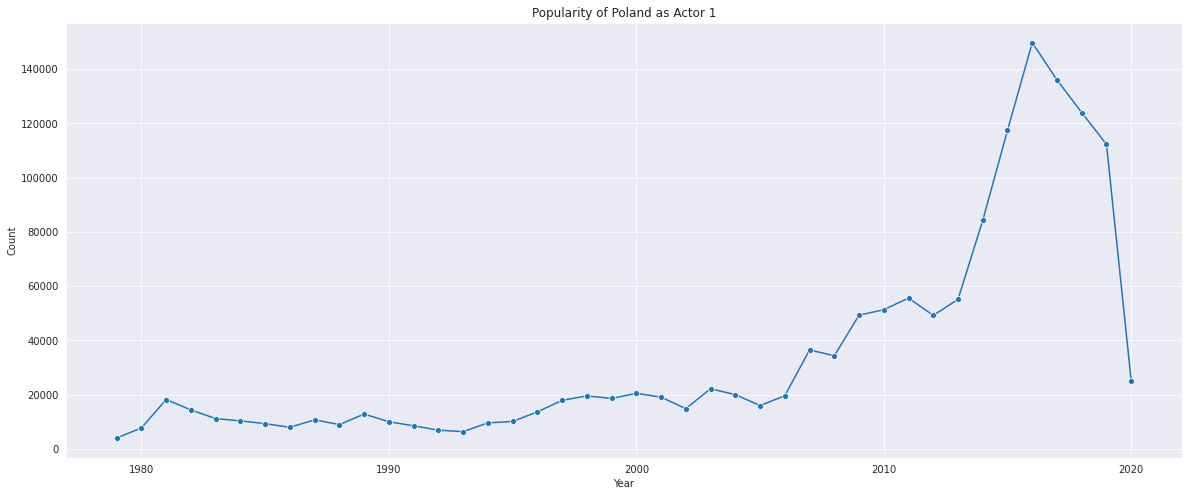
\includegraphics[width=1 \textwidth]{fig/PL/PLactor1.png}
        \caption{Ilość zdarzeń z Polską jako aktorem 1. (źródło: opracowanie własne)}
        \label{fig:PLactor1}
        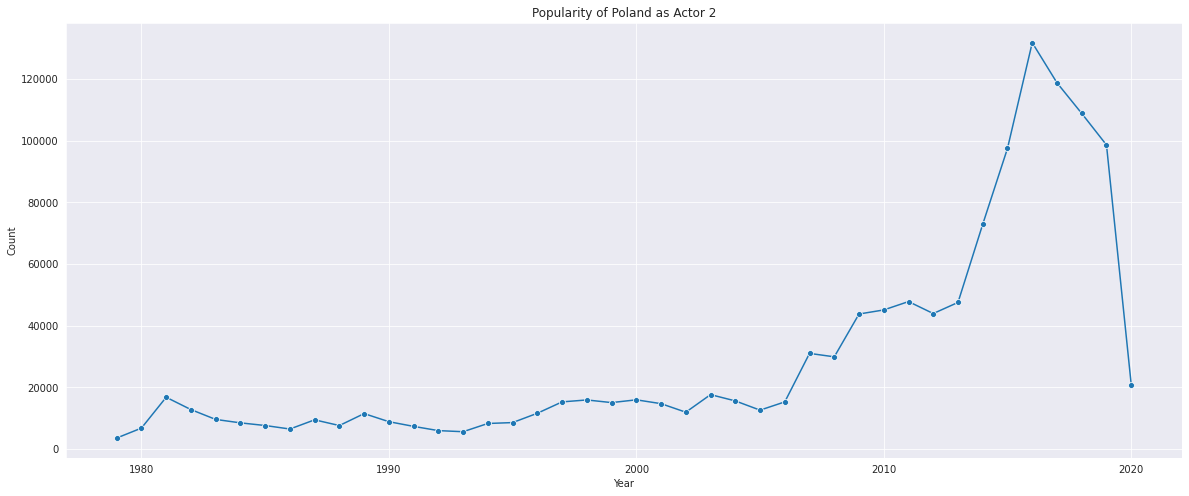
\includegraphics[width=1 \textwidth]{fig/PL/PLactor2.png}
        \caption{Ilość zdarzeń z Polską jako aktorem 2. (źródło: opracowanie własne)}
        \label{fig:PLactor2}
    \end{figure}

    \paragraph{Polska jako Aktor 2}
    Wykers~\ref{fig:PLactor2} przedstawia popularność Polski jako aktora 2 skumulowaną dla poszczególnych lat. Kształt wykresu jest bardzo zbliżony do~\ref{fig:PLactor1} jednak szczyt popularności jest niższy - na poziomie około 130 tysięcy zdarzeń.

    \paragraph{Polska jako miejsce wydarzeń}
    Wykers~\ref{fig:PLlocation} przedstawia popularność Polski jako miejsca wydarzeń skumulowaną dla poszczególnych lat. Ponownie kształt wykresu jest zbliżony do~\ref{fig:PLactor1}. W tym przypadku szczyt popularności jest wyższy - na poziomie około 210 tysięcy zdarzeń.
    \begin{figure}[ht!]
        \centering
        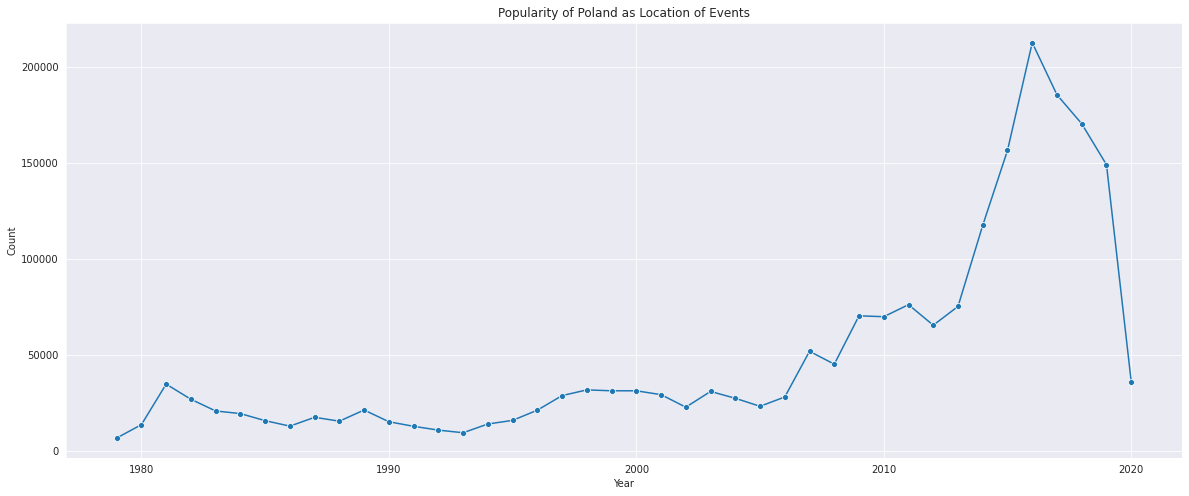
\includegraphics[width=1 \textwidth]{fig/PL/PLlocation.png}
        \caption{Ilość zdarzeń z Polską jako lokacją. (źródło: opracowanie własne)}
        \label{fig:PLlocation}
    \end{figure}

    \subsection{Analiza zbiorcza od 2015 roku}
    Dane pochodzą z przedziału od stycznia 2015 do kwietnia 2020 roku.

    \paragraph{Ilość zdarzeń dla poszczególnych krajów}
    Wykres~\ref{fig:GLOBALactor1} przedstawia sumaryczną ilość zdarzeń od 2015 roku, dla poszczególnych krajów, uszeregowaną malejąco.
    \begin{figure}[ht!]
        \centering
        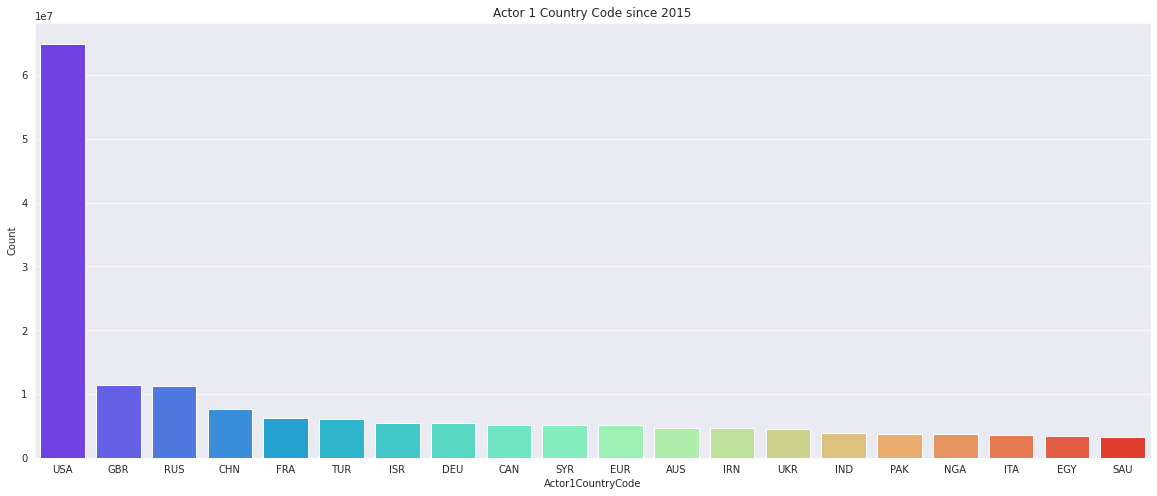
\includegraphics[width=1 \textwidth]{fig/GLOBAL/Actor1.png}
        \caption{Ilość zdarzeń dla poszczególnych krajów. (źródło: opracowanie własne)}
        \label{fig:GLOBALactor1}
    \end{figure}
    Niekwestionowanym liderem pod względem ilości zdarzeń są Stany Zjednoczone. Dystansują one pozostałe kraje o prawie rząd wielkości. Kraje anglosaskie są szczeegolnie mocno reprezentowane. W czołówce pojawiają sie też kraje znaczace polictycznie oraz silnie skonfliktowane.

    \paragraph{Ilość zdarzeń w czasie}
    Wykres~\ref{fig:GLOBALactor1inTime} przedstawia ilość zdarzeń dla top 5 krajów skumulowaną dla poszczególnych lat.
    WYKRES DO POPRAWY
    \begin{figure}[ht!]
        \centering
        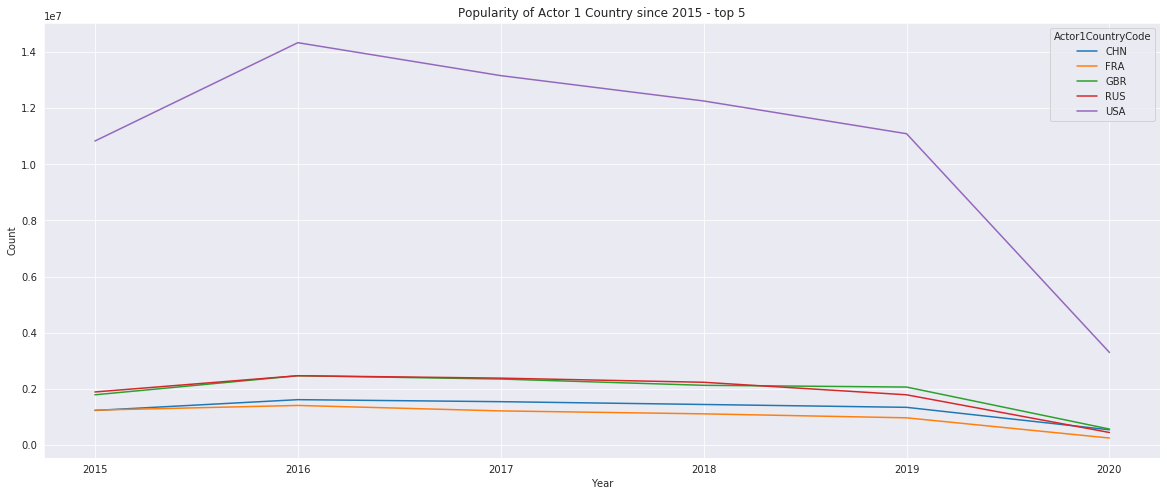
\includegraphics[width=1 \textwidth]{fig/GLOBAL/Actor1inTIME.png}
        \caption{Ilość zdarzeń dla poszczególnych krajów w czasie. (źródło: opracowanie własne)}
        \label{fig:GLOBALactor1inTime}
    \end{figure}

    \paragraph{Popularność czterokodów zdarzeń}
    Wykres~\ref{fig:GLOBALQC} przedstawia sumaryczną ilość zdarzeń od 2015 roku, dla poszczególnych czterokodów zdarzeń, uszeregowaną malejąco.
    \begin{figure}[ht!]
        \centering
        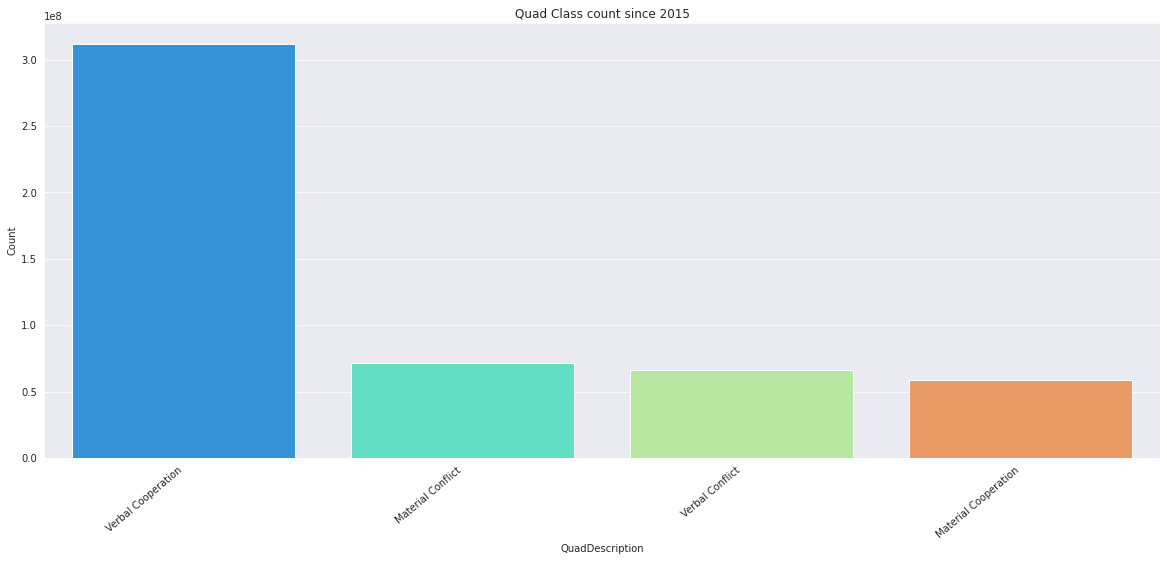
\includegraphics[width=1 \textwidth]{fig/GLOBAL/QC.png}
        \caption{Ilość zdarzeń dla poszczególnych kodów w czasie. (źródło: opracowanie własne)}
        \label{fig:GLOBALQC}
    \end{figure}

    \paragraph{Popularność czterokodów zdarzeń w czasie}
    Wykres~\ref{fig:GLOBALQCperc} przedstawia ilość zdarzeń dla czterokodów zdarzeń skumulowaną dla poszczególnych lat.
    WYKRES DO POPRAWY
    \begin{figure}[ht!]
        \centering
        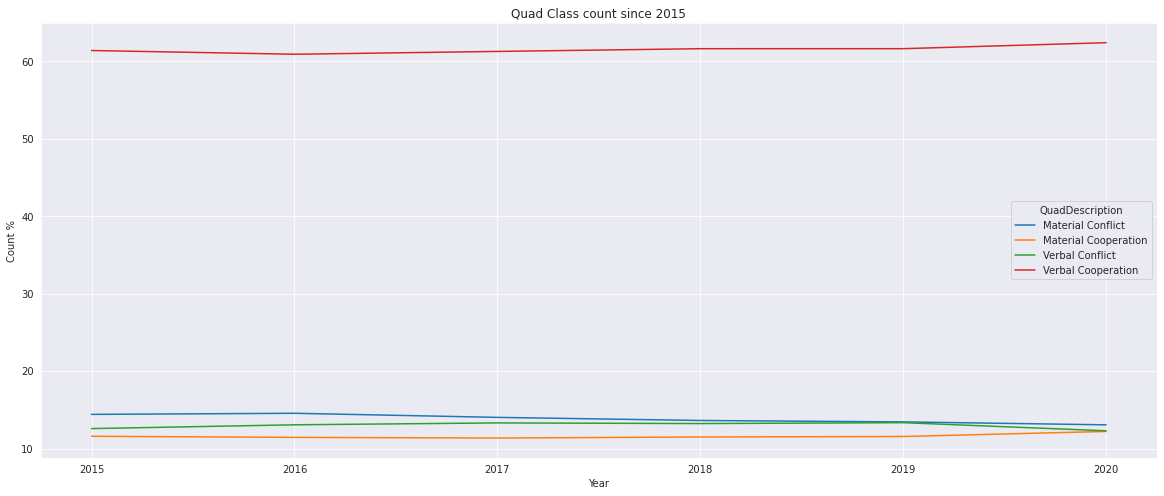
\includegraphics[width=1 \textwidth]{fig/GLOBAL/QCperc.png}
        \caption{Procentowa ilość zdarzeń dla poszczególnych kodów w czasie. (źródło: opracowanie własne)}
        \label{fig:GLOBALQCperc}
    \end{figure}

    \paragraph{Popularność bazowych kodów zdarzeń}
    Wykres~\ref{fig:GLOBALEBC} przedstawia sumaryczną ilość zdarzeń od 2015 roku, dla poszczególnych bazowych kodów zdarzeń, uszeregowaną malejąco.
    \begin{figure}[ht!]
        \centering
        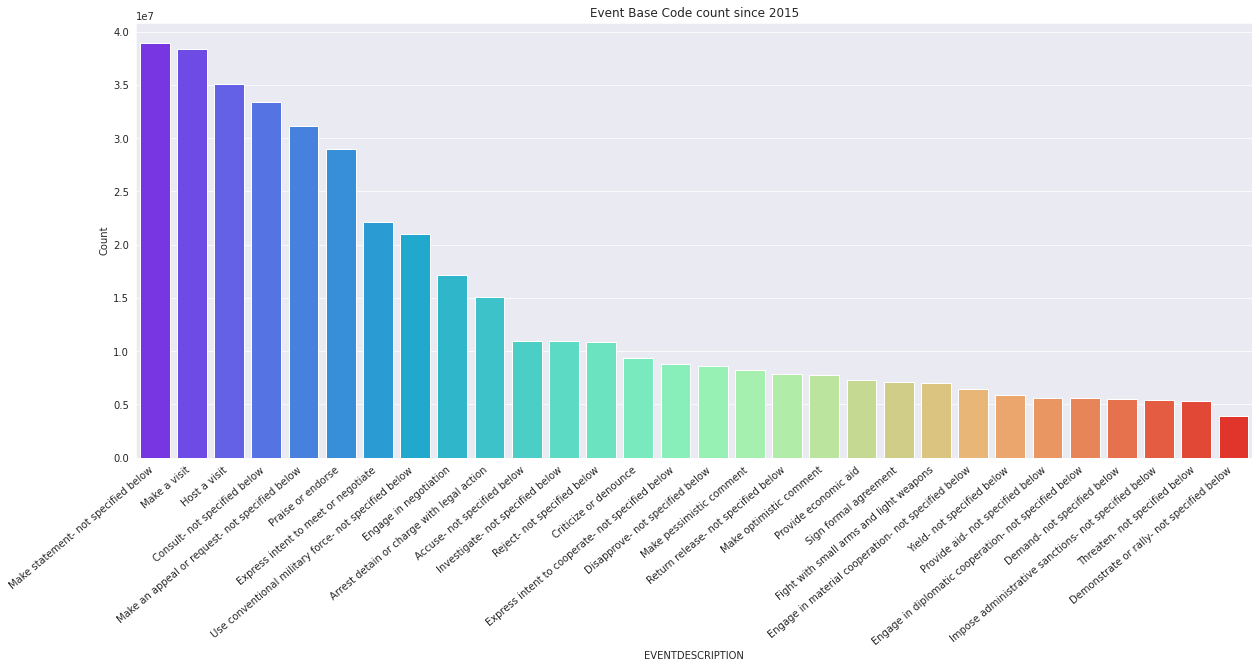
\includegraphics[width=1 \textwidth]{fig/GLOBAL/EBC.png}
        \caption{Ilość zdarzeń dla poszczególnych kodów w czasie. (źródło: opracowanie własne)}
        \label{fig:GLOBALEBC}
    \end{figure}

    \paragraph{Popularność bazowych kodów zdarzeń w czasie}
    Wykres~\ref{fig:GLOBALEBCperc} przedstawia ilość zdarzeń dla top 20 bazowych kodów zdarzeń skumulowaną dla poszczególnych lat.
    WYKRES DO POPRAWY
    \begin{figure}[ht!]
        \centering
        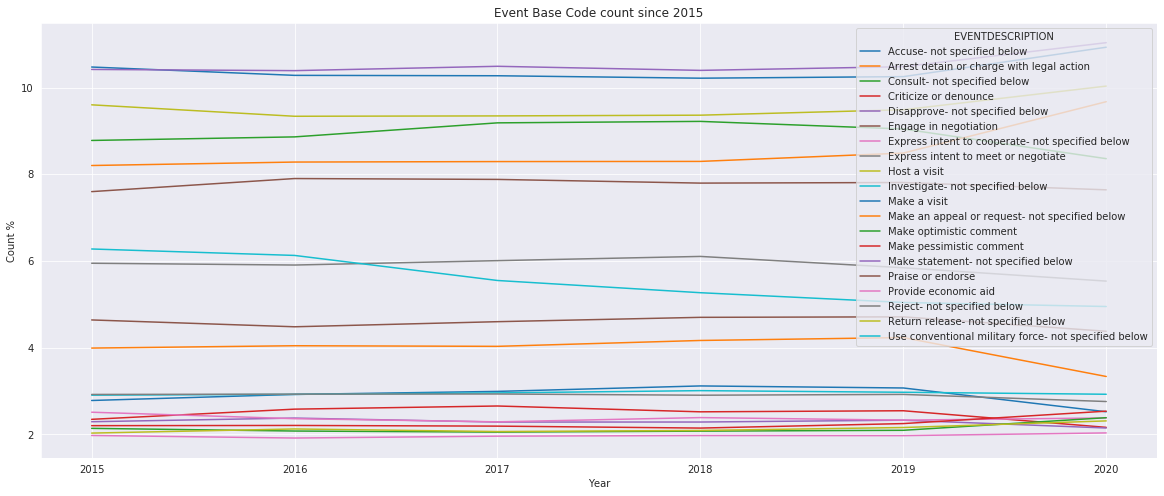
\includegraphics[width=1 \textwidth]{fig/GLOBAL/EBCperc.png}
        \caption{Procentowa ilość zdarzeń dla poszczególnych kodów w czasie. (źródło: opracowanie własne)}
        \label{fig:GLOBALEBCperc}
    \end{figure}

    \paragraph{Popularność podstawowych kodów zdarzeń}
    Wykres~\ref{fig:GLOBALERC} przedstawia sumaryczną ilość zdarzeń od 2015 roku, dla poszczególnych podstawowych kodów zdarzeń, uszeregowaną malejąco.
    \begin{figure}[ht!]
        \centering
        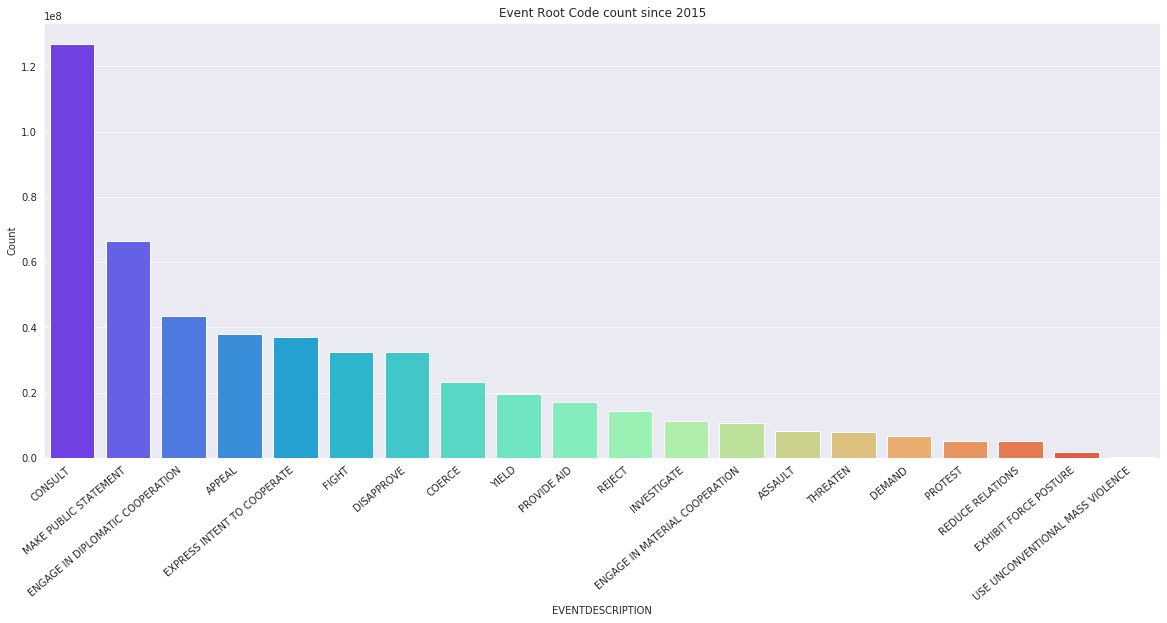
\includegraphics[width=1 \textwidth]{fig/GLOBAL/ERC.png}
        \caption{Ilość zdarzeń dla poszczególnych kodów w czasie. (źródło: opracowanie własne)}
        \label{fig:GLOBALERC}
    \end{figure}

    \paragraph{Popularność podstawowych kodów zdarzeń w czasie}
    Wykres~\ref{fig:GLOBALERCperc} przedstawia ilość zdarzeń dla top 20 podstawowych kodów zdarzeń skumulowaną dla poszczególnych lat.
    WYKRES DO POPRAWY
    \begin{figure}[ht!]
        \centering
        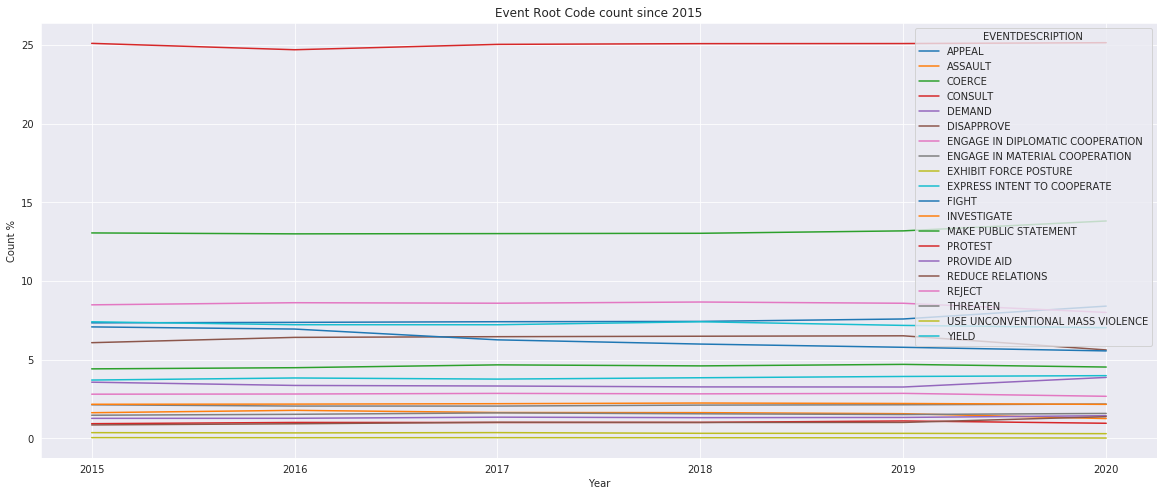
\includegraphics[width=1 \textwidth]{fig/GLOBAL/ERCperc.png}
        \caption{Procentowa ilość zdarzeń dla poszczególnych kodów w czasie. (źródło: opracowanie własne)}
        \label{fig:GLOBALERCperc}
    \end{figure}


    \section{Analiza danych dla wybranych krajów}

    \subsection{Polska}

    \paragraph{Kraj para do zdarzenia}


    Wykres~\ref{fig:PLpair} przedstawia ilość zdarzeń dla Polski w których parą jest dany kraj.

    \begin{figure}[ht!]
        \centering
        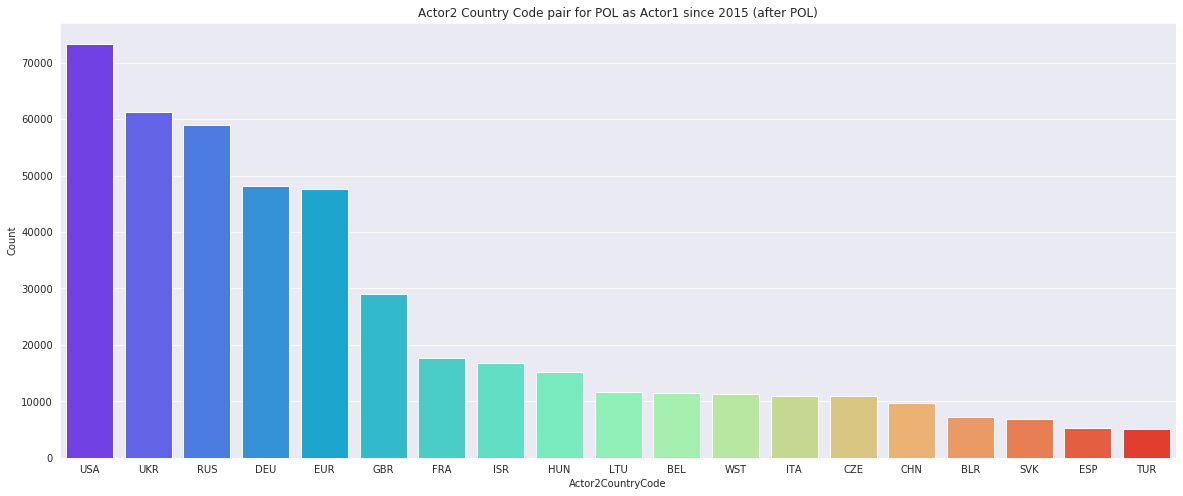
\includegraphics[width=1 \textwidth]{fig/PL/PLactor2Pair.png}
        \caption{Ilość zdarzeń w których parą jest dany kraj. (źródło: opracowanie własne)}
        \label{fig:PLpair}
    \end{figure}


    Wykres~\ref{fig:PLpairPerc} przedstawia ilość zdarzeń dla Polski w których parą jest dany kraj w czasie.

    WYKRES DO POPRAWY
    \begin{figure}[ht!]
        \centering
        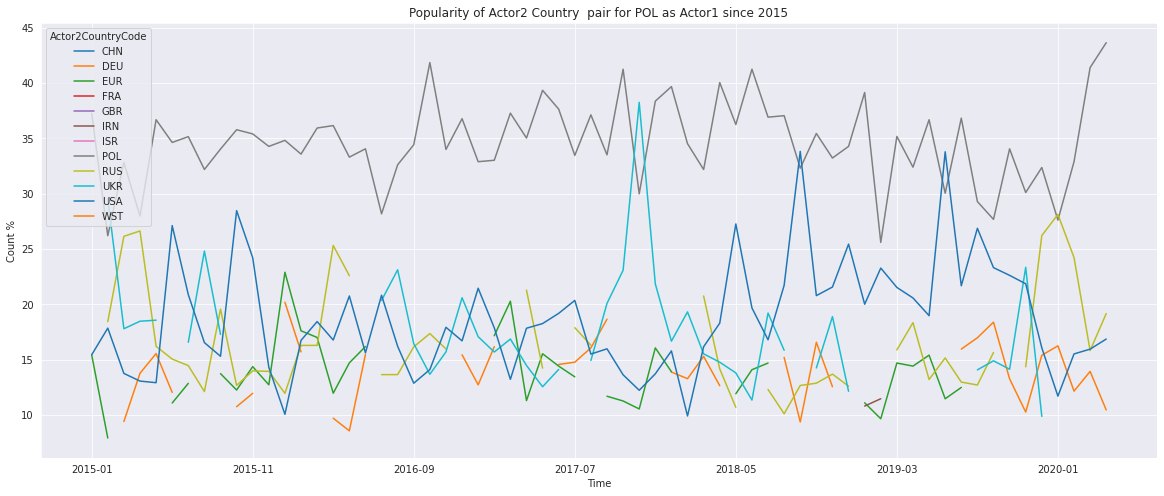
\includegraphics[width=1 \textwidth]{fig/PL/PLactor2PairPercinTIME.png}
        \caption{Procentowa ilość zdarzeń w których parą jest dany kraj w czasie. (źródło: opracowanie własne)}
        \label{fig:PLpairPerc}
    \end{figure}

    \paragraph{Podstawowy kod zdarzeń}

    Wykres~\ref{fig:PLPERC} przedstawia ilość zdarzeń dla Polski dla poszczególnych kodów podstawowych.


    \begin{figure}[ht!]
        \centering
        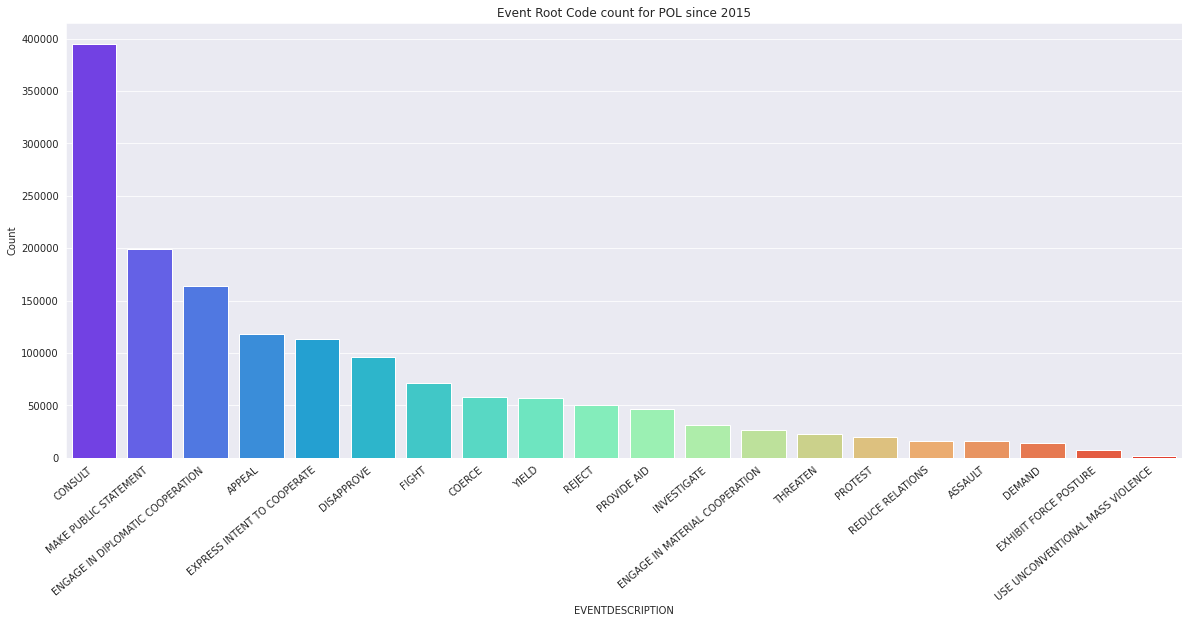
\includegraphics[width=1 \textwidth]{fig/PL/PLERC.png}
        \caption{Ilość zdarzeń dla poszczególnych kodów podstawowocy. (źródło: opracowanie własne)}
        \label{fig:PLPERC}
    \end{figure}

    Wykres~\ref{fig:PLPERCinTIME} przedstawia ilość zdarzeń dla Polski dla poszczególnych kodów podstawowych w czasie.

    WYKRES DO POPRAWY
    \begin{figure}[ht!]
        \centering
        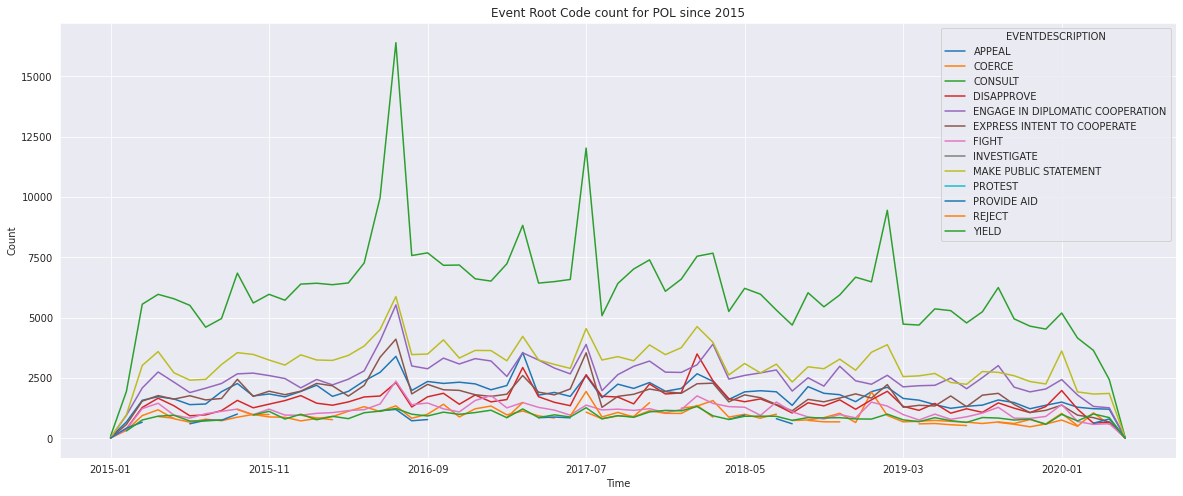
\includegraphics[width=1 \textwidth]{fig/PL/PLERCinTIME.png}
        \caption{Ilość zdarzeń dla poszczególnych kodów podstawowocy w czasie. (źródło: opracowanie własne)}
        \label{fig:PLPERCinTIME}
    \end{figure}

    Wykres~\ref{fig:PLPERCpercinTIME} przedstawia procentową ilość zdarzeń dla Polski dla poszczególnych kodów podstawowych w czasie.

    WYKRES DO POPRAWY
    \begin{figure}[ht!]
        \centering
        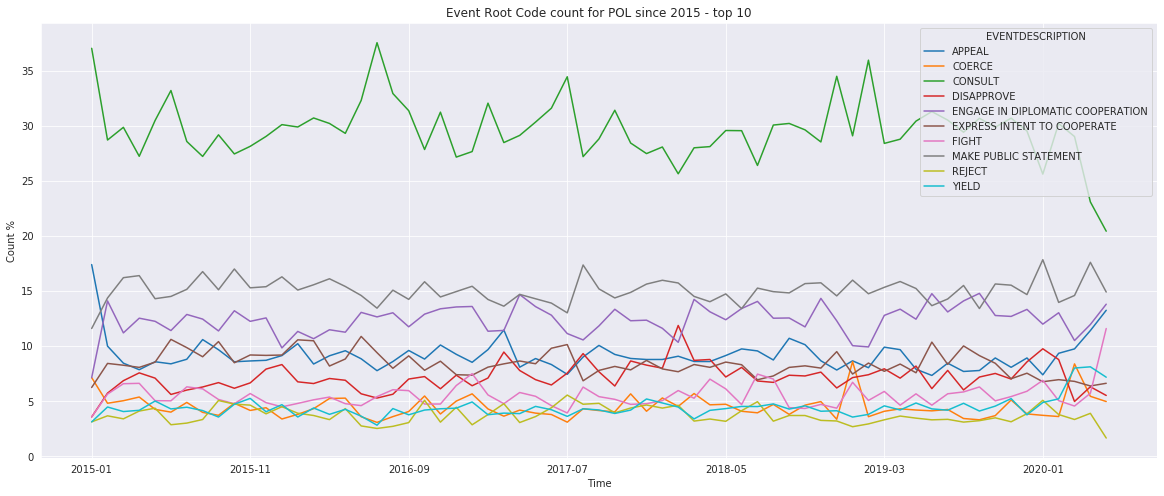
\includegraphics[width=1 \textwidth]{fig/PL/PLERCpercinTIME.png}
        \caption{Procentowa ilość zdarzeń dla poszczególnych kodów podstawowocy w czasie. (źródło: opracowanie własne)}
        \label{fig:PLPERCpercinTIME}
    \end{figure}

    \paragraph{Podstawowe kody zdarzeń między Polską a wybranymi krajami}

    Wykres~\ref{fig:PLDEUERC} przedstawia ilość zdarzeń z Niemcami dla poszczególnych kodów podstawowocy w czasie.

    WYKRES DO POPRAWY
    \begin{figure}[ht!]
        \centering
        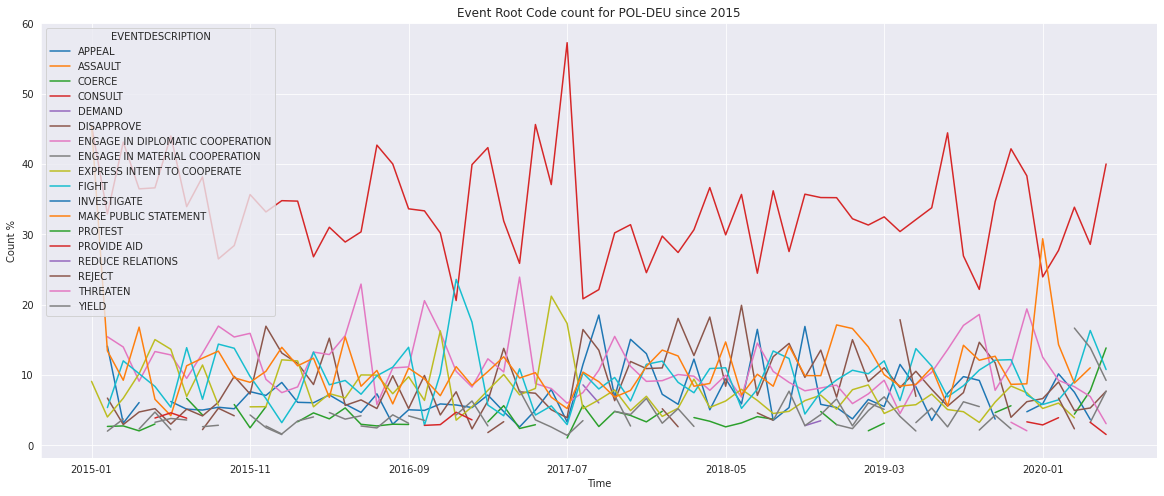
\includegraphics[width=1 \textwidth]{fig/PL/POLDEUERCperc.png}
        \caption{Procentowa ilość zdarzeń z Niemcami dla poszczególnych kodów podstawowocy w czasie. (źródło: opracowanie własne)}
        \label{fig:PLDEUERC}
    \end{figure}

    Wykres~\ref{fig:PLFRAERC} przedstawia ilość zdarzeń z Francją dla poszczególnych kodów podstawowocy w czasie.


    WYKRES DO POPRAWY
    \begin{figure}[ht!]
        \centering
        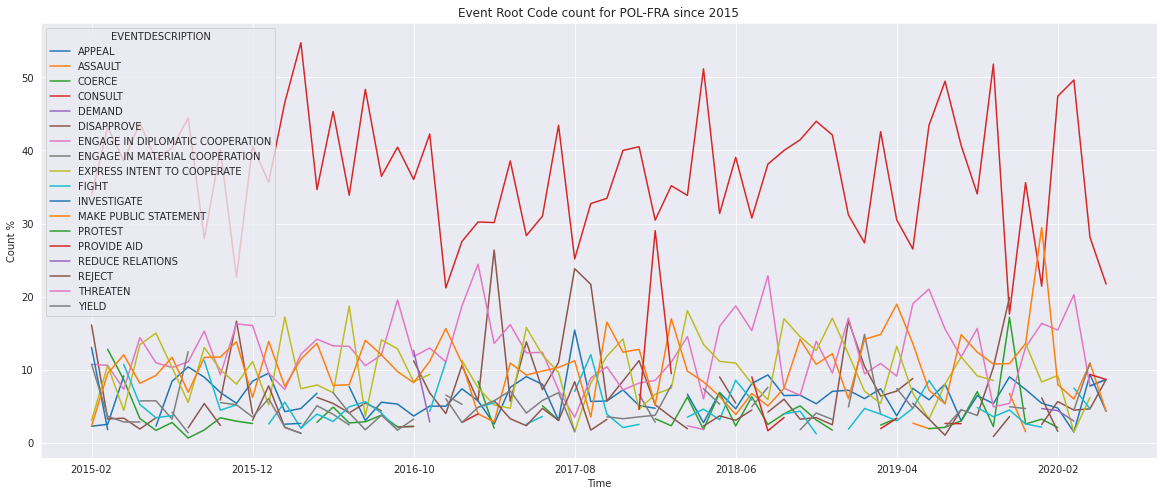
\includegraphics[width=1 \textwidth]{fig/PL/POLFRAERCperc.png}
        \caption{Procentowa ilość zdarzeń z Francją dla poszczególnych kodów podstawowocy w czasie. (źródło: opracowanie własne)}
        \label{fig:PLFRAERC}
    \end{figure}

    Wykres~\ref{fig:PLGBRERC} przedstawia ilość zdarzeń z Wielką Brytanią dla poszczególnych kodów podstawowocy w czasie.

    WYKRES DO POPRAWY
    \begin{figure}[ht!]
        \centering
        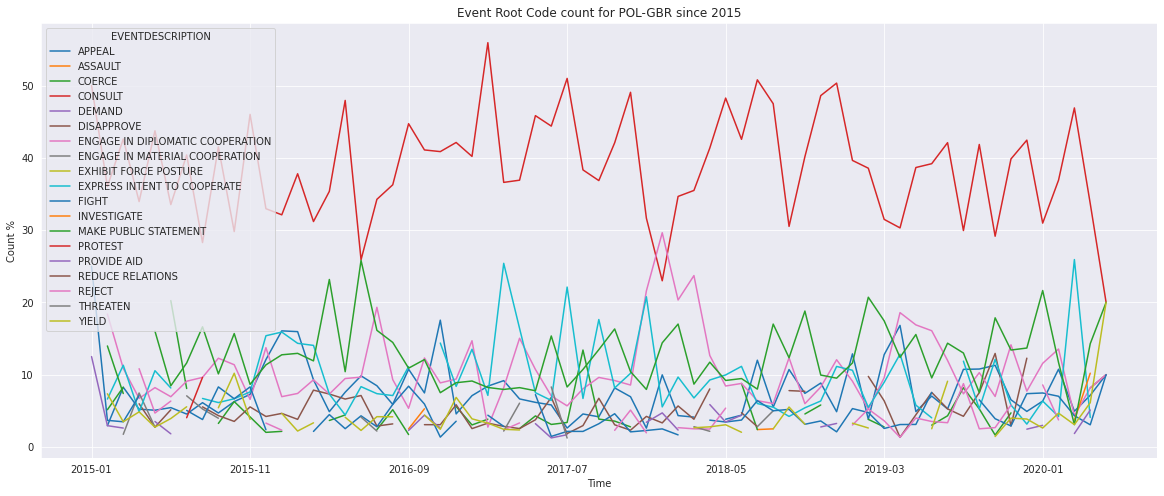
\includegraphics[width=1 \textwidth]{fig/PL/POLGBRERCperc.png}
        \caption{Procentowa ilość zdarzeń z Wielka Brytanią dla poszczególnych kodów podstawowocy w czasie. (źródło: opracowanie własne)}
        \label{fig:PLGBRERC}
    \end{figure}

    Wykres~\ref{fig:PLRUSERC} przedstawia ilość zdarzeń z Rosją dla poszczególnych kodów podstawowocy w czasie.

    WYKRES DO POPRAWY
    \begin{figure}[ht!]
        \centering
        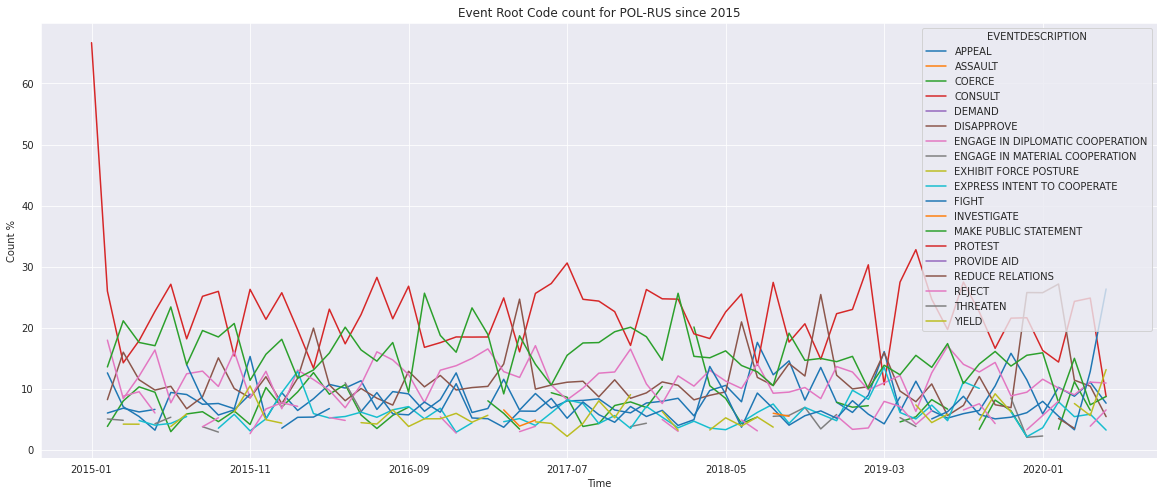
\includegraphics[width=1 \textwidth]{fig/PL/POLRUSERCperc.png}
        \caption{Procentowa ilość zdarzeń z Rosją dla poszczególnych kodów podstawowocy w czasie. (źródło: opracowanie własne)}
        \label{fig:PLRUSERC}
    \end{figure}

    \subsection{Niemcy}

    \subsection{Rosja}

    \subsection{Stan zjednoczone}

    \subsection{Pozostałe}


    \section{Analiza siły powiązania}

    \subsection{Analiza siły powiązania miedzy wybranymi krajami}

    \paragraph{Polska}

    Wykres~\ref{fig:PLConnection} przedstawia siłę połączenia Polski z wybranaymi krajami w czasie.


    \begin{figure}[ht!]
        \centering
        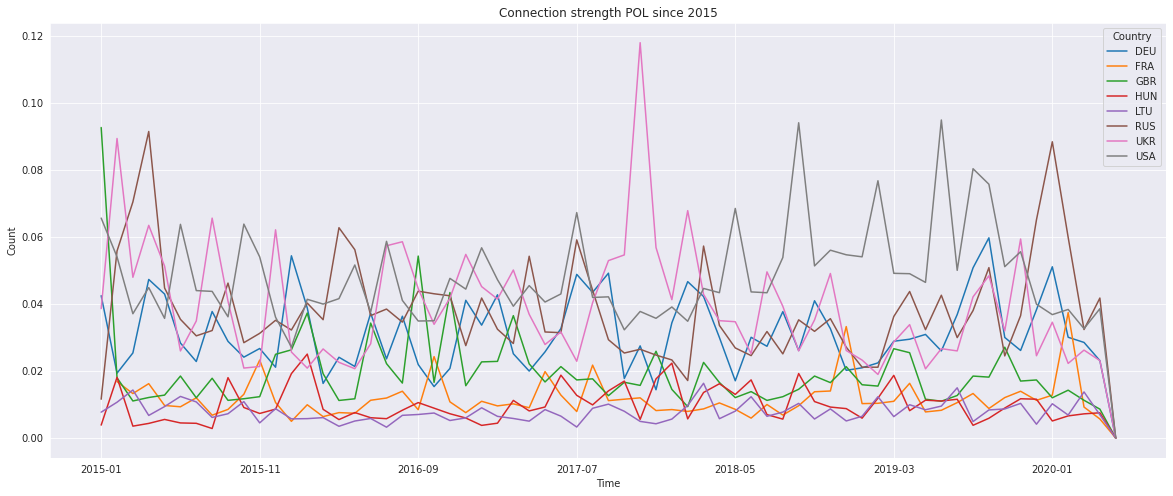
\includegraphics[width=1 \textwidth]{fig/PL/POLConnection.png}
        \caption{Siła połączenia Polski z wybranymi krajami w czasie. (źródło: opracowanie własne)}
        \label{fig:PLConnection}
    \end{figure}

    \paragraph{Rosja}

    Wykres~\ref{fig:RUSConnection} przedstawia siłę połączenia Rosji z wybranaymi krajami w czasie.

    \begin{figure}[ht!]
        \centering
        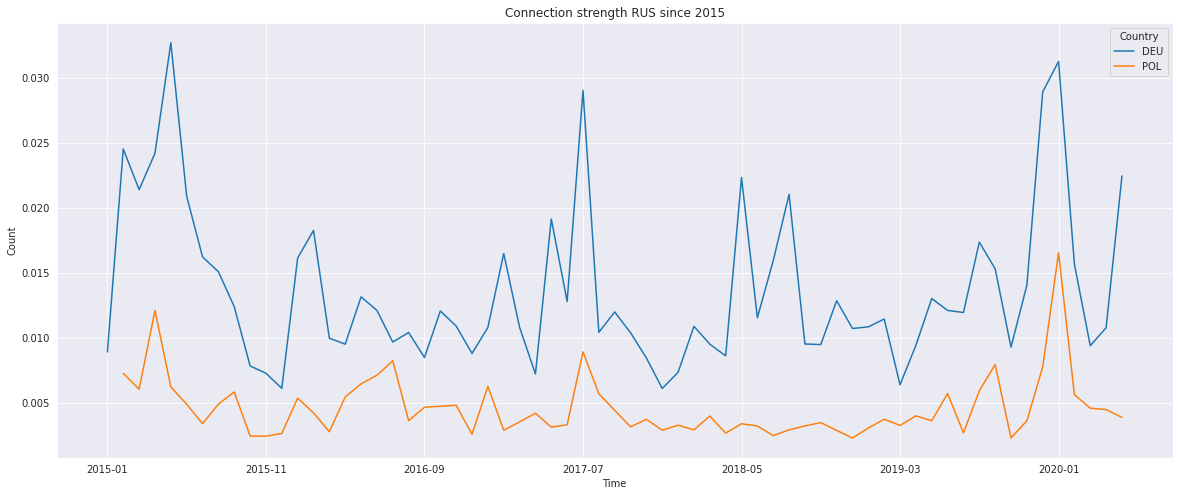
\includegraphics[width=1 \textwidth]{fig/RUS/RUSConnection.png}
        \caption{Siła połączenia Rosji z wybranymi krajami w czasie. (źródło: opracowanie własne)}
        \label{fig:RUSConnection}
    \end{figure}

    \paragraph{Niemcy}

    Wykres~\ref{fig:DEUConnection} przedstawia siłę połączenia Niemiec z wybranaymi krajami w czasie.

    \begin{figure}[ht!]
        \centering
        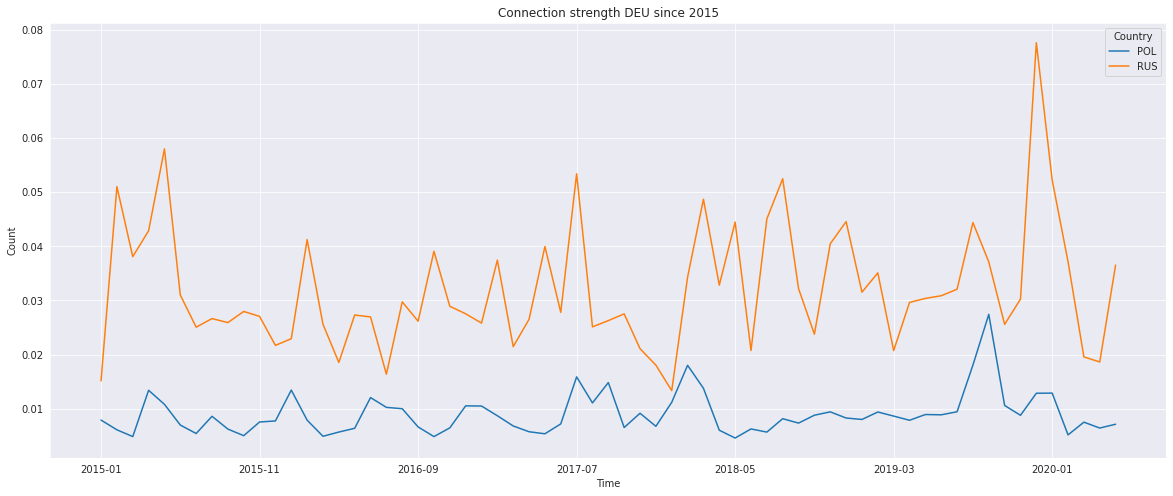
\includegraphics[width=1 \textwidth]{fig/DEU/DEUConnection.png}
        \caption{Siła połączenia Niemiec z wybranymi krajami w czasie. (źródło: opracowanie własne)}
        \label{fig:DEUConnection}
    \end{figure}

    \paragraph{Stany Zjednoczone}

    Wykres~\ref{fig:PLConnection} przedstawia siłę połączenia Stanów Zjednoczonych z wybranaymi krajami w czasie.

    \begin{figure}[ht!]
        \centering
        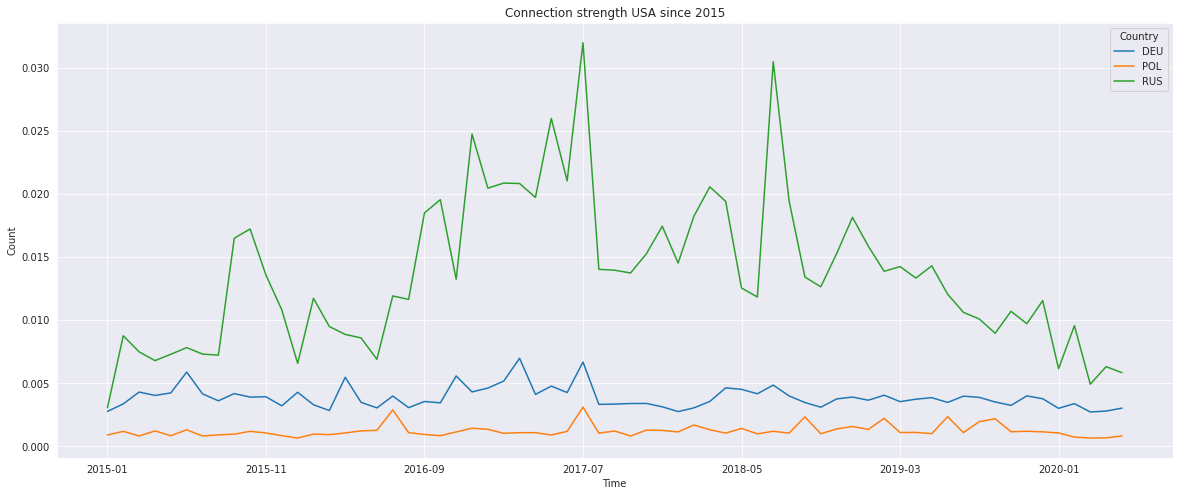
\includegraphics[width=1 \textwidth]{fig/USA/USAConnection.png}
        \caption{Siła połączenia Stanów Zjednoczonych z wybranymi krajami w czasie. (źródło: opracowanie własne)}
        \label{fig:USAConnection}
    \end{figure}

    \subsection{Analiza symetryczności siły powiązania}

    \paragraph{Polska - Niemcy - Polska}

    Wykres~\ref{fig:POL-DEU-POL} przedstawia symetryczność siły połączenia Polski i Niemiec w czasie.


    \begin{figure}[ht!]
        \centering
        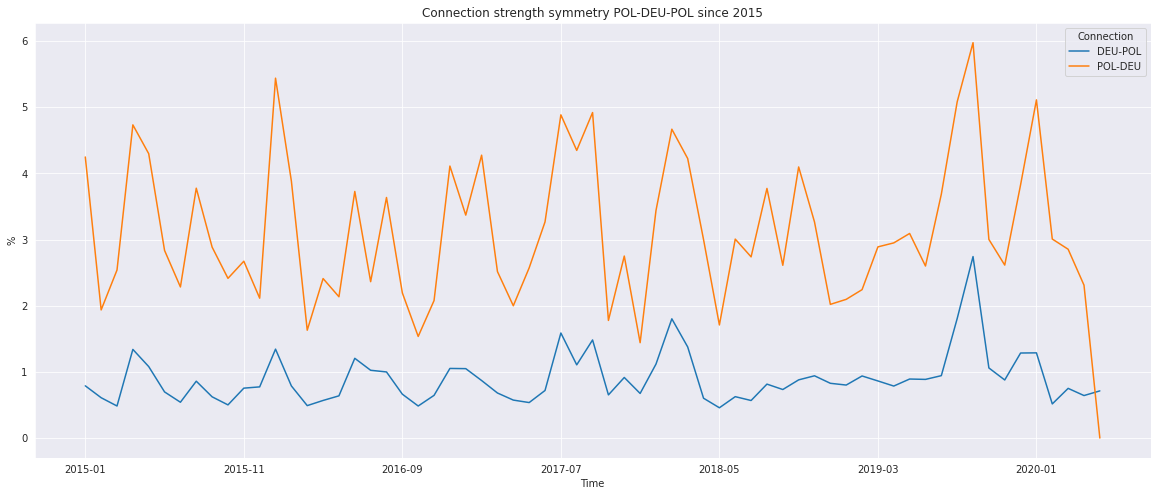
\includegraphics[width=1 \textwidth]{fig/ConnectionSymmetry/POL-DEU-POL.png}
        \caption{Symetryczność siły połączenia Polski i Niemiec w czasie. (źródło: opracowanie własne)}
        \label{fig:POL-DEU-POL}
    \end{figure}

    \paragraph{Polska - Rosja - Polska}

    Wykres~\ref{fig:POL-RUS-POL} przedstawia symetryczność siły połączenia Polski i Rosji w czasie.


    \begin{figure}[ht!]
        \centering
        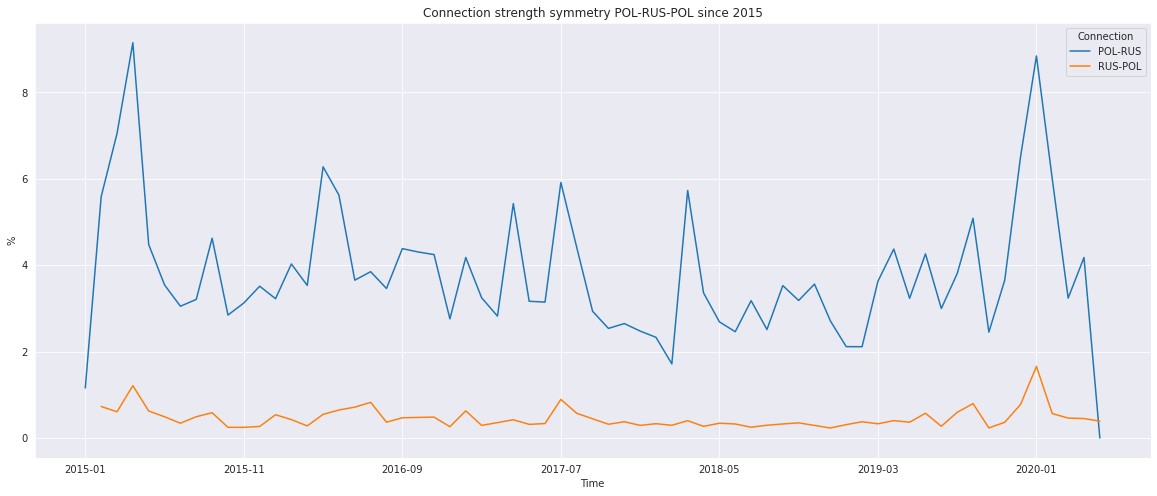
\includegraphics[width=1 \textwidth]{fig/ConnectionSymmetry/POL-RUS-POL.png}
        \caption{Symetryczność siły połączenia Polski i Rosji w czasie. (źródło: opracowanie własne)}
        \label{fig:POL-RUS-POL}
    \end{figure}

    \paragraph{Polska - Stany Zjednoczone - Polska}

    Wykres~\ref{fig:POL-USA-POL} przedstawia symetryczność siły połączenia Polski i Stanów Zjednoczonych w czasie.


    \begin{figure}[ht!]
        \centering
        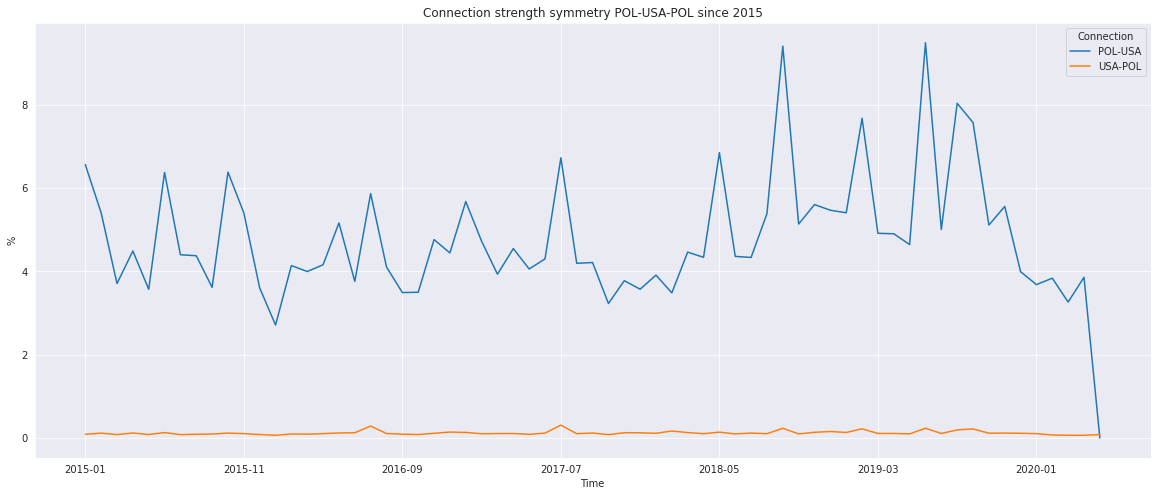
\includegraphics[width=1 \textwidth]{fig/ConnectionSymmetry/POL-USA-POL.png}
        \caption{Symetryczność siły połączenia Polski i Stanów Zjednoczonych w czasie. (źródło: opracowanie własne)}
        \label{fig:POL-USA-POL}
    \end{figure}


    \section{Analiza wybranych kodów podstawowych}

    \subsection{Fight}

    Wykres~\ref{fig:Fight} przedstawia procentową ilość państw z jakimi dany kraj ma zdarzenia fight w czasie.


    \begin{figure}[ht!]
        \centering
        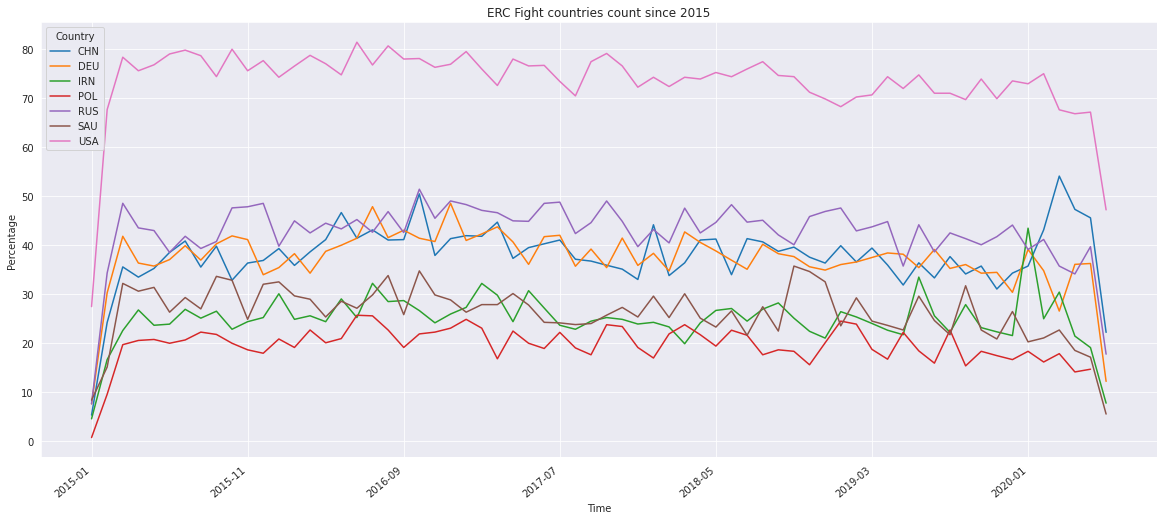
\includegraphics[width=1 \textwidth]{fig/ERC/Fight.png}
        \caption{Procentowa ilość państw z jakimi dany kraj ma zdarzenia fight w czasie. (źródło: opracowanie własne)}
        \label{fig:Fight}
    \end{figure}

    \subsection{Express intent to cooperate}

    Wykres\ldots przedstawia procentową ilość państw z jakimi dany kraj ma zdarzenia fight w czasie.


    \section{Analiza średniego tonu wydarzeń dla wybranych krajów}


    \section{Analiza miary Goldsteina wydarzeń dla wybranych krajów}


    \section{Klasteryzacja}

    \subsection{Grupowanie z wykorzystaniem K-Means - 10 klastrów}

    Do przeprowadzenia pierwszego grupowania krajów wykorzystany został wektor składający się z:
    \begin{enumerate}
        \item[•] ilości zdarzeń dla których kraj jest aktorem 1
        \item[•] ilości wzmianek (numMentions)
        \item[•] ilości material conflict/cooperation z quad description
        \item[•] ilości verbal conflict/cooperation z quad description
        \item[•] średniego średniego tonu
        \item[•] średniej miary Goldsteina
        \item[•] ilości zdarzeń Fight
        \item[•] ilości zdarzeń Express intent to cooperate
    \end{enumerate}
    Dane wykorzystane w tym doświadczeniu pochodzą ze stycznia 2020 roku.
    Przed dokonaniem klasteryzacji odrzucone zostały wydarzenia z kodami krajów cameo niezgodnymi z kodami ISO 3166-1 alfa-3~\cite{iso_alfa3}.
    Klasteryzacja została przeprowadzona dwukrotnie, za drugim razem na danych ustandaryzowanych przy pomocy modułu StandardScaler~\cite{standardScaler}.

    \subsubsection{Dane niestandaryzowane}
    W pierwszej kolejności zostaną przedstawione wyniki grupowania na danych niestandaryzowanych.

    Wykres~\ref{fig:clust10} przedstawia mapę z naniesionymi wynikami klasteryzacji. Każda grupa krajów otrzymała inny kolor.

    \begin{figure}[ht!]
        \centering
        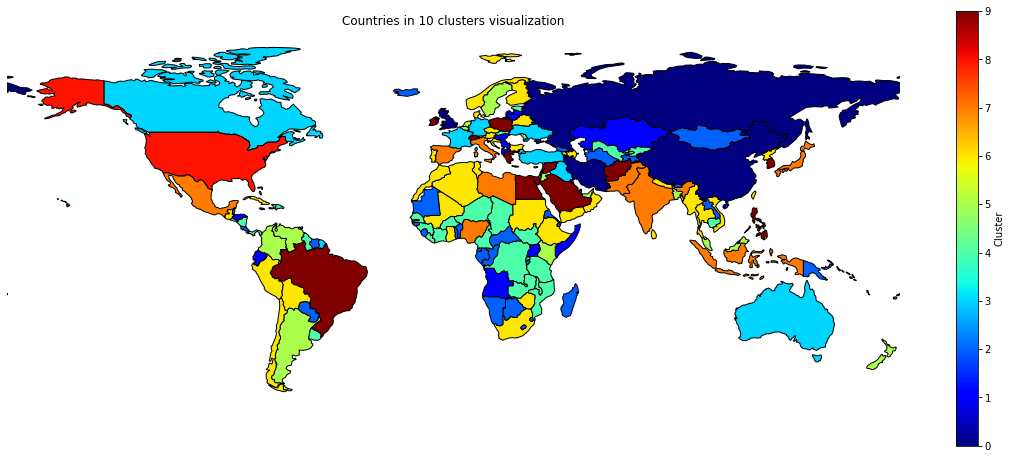
\includegraphics[width=1 \textwidth]{fig/CLUST/10clusterMap.png}
        \caption{Mapa z wynikami klasteryzacji. (źródło: opracowanie własne)}
        \label{fig:clust10}
    \end{figure}

    \paragraph{Wyniki klasteryzacji w postaci tabelarycznej}
    W tabelach od~\ref{tab:cl0} do~\ref{tab:cl9} przedstawione zostały wyniki grupowania.
    Dodatkowo zawarto informacje o ilości ludności i PKB na osobę pochodzące z biblioteki GeoPandas~\cite{geopandas}.

    \begin{table}[h!]
        \caption {Klaster 0} \label{tab:cl0}
        \begin{tabular}{lllll}
            \hline
            \multicolumn{1}{|l|}{iso\_a3} & \multicolumn{1}{l|}{name} & \multicolumn{1}{l|}{continent} & \multicolumn{1}{l|}{pop\_est} & \multicolumn{1}{l|}{gdp\_per\_cap} \\ \hline
            DZA                           & Algeria                   & Africa                         & 40969443                      & 0.014875                           \\
            ARM                           & Armenia                   & Asia                           & 3045191                       & 0.008637                           \\
            AUT                           & Austria                   & Europe                         & 8754413                       & 0.047587                           \\
            AZE                           & Azerbaijan                & Asia                           & 9961396                       & 0.016855                           \\
            BLR                           & Belarus                   & Europe                         & 9549747                       & 0.017320                           \\
            BOL                           & Bolivia                   & South America                  & 11138234                      & 0.007034                           \\
            BGR                           & Bulgaria                  & Europe                         & 7101510                       & 0.020151                           \\
            CHL                           & Chile                     & South America                  & 17789267                      & 0.024515                           \\
            HRV                           & Croatia                   & Europe                         & 4292095                       & 0.021957                           \\
            CUB                           & Cuba                      & North America                  & 11147407                      & 0.011922                           \\
            CYP                           & Cyprus                    & Asia                           & 1221549                       & 0.023953                           \\
            CYP                           & Cyprus                    & Asia                           & 1221549                       & 0.023953                           \\
            CZE                           & Czechia                   & Europe                         & 10674723                      & 0.032872                           \\
            DNK                           & Denmark                   & Europe                         & 5605948                       & 0.047236                           \\
            ETH                           & Ethiopia                  & Africa                         & 105350020                     & 0.001658                           \\
            FIN                           & Finland                   & Europe                         & 5491218                       & 0.040817                           \\
            GHA                           & Ghana                     & Africa                         & 27499924                      & 0.004393                           \\
            GTM                           & Guatemala                 & North America                  & 15460732                      & 0.008525                           \\
            MLI                           & Mali                      & Africa                         & 17885245                      & 0.002130                           \\
            MAR                           & Morocco                   & Africa                         & 33986655                      & 0.008321                           \\
            MMR                           & Myanmar                   & Asia                           & 55123814                      & 0.005644                           \\
            CYP                           & N. Cyprus                 & Asia                           & 265100                        & 0.013580                           \\
            CYP                           & N. Cyprus                 & Asia                           & 265100                        & 0.013580                           \\
            NPL                           & Nepal                     & Asia                           & 29384297                      & 0.002434                           \\
            PRK                           & North Korea               & Asia                           & 25248140                      & 0.001584                           \\
            NOR                           & Norway                    & Europe                         & 5320045                       & 0.068552                           \\
            OMN                           & Oman                      & Asia                           & 3424386                       & 0.050549                           \\
            PER                           & Peru                      & South America                  & 31036656                      & 0.013223                           \\
            PRT                           & Portugal                  & Europe                         & 10839514                      & 0.027409                           \\
            ZAF                           & South Africa              & Africa                         & 54841552                      & 0.013477                           \\
            LKA                           & Sri Lanka                 & Asia                           & 22409381                      & 0.010563                           \\
            SDN                           & Sudan                     & Africa                         & 37345935                      & 0.004721                           \\
            TWN                           & Taiwan                    & Asia                           & 23508428                      & 0.047940                           \\
            THA                           & Thailand                  & Asia                           & 68414135                      & 0.016970                           \\
            TUN                           & Tunisia                   & Africa                         & 11403800                      & 0.011470                           \\
            VNM                           & Vietnam                   & Asia                           & 96160163                      & 0.006187                           \\
            YEM                           & Yemen                     & Asia                           & 28036829                      & 0.002620                           \\
            ZWE                           & Zimbabwe                  & Africa                         & 13805084                      & 0.002052
        \end{tabular}
    \end{table}

    \begin{table}[h!]
        \caption {Klaster 1} \label{tab:cl1}
        \begin{tabular}{lllll}
            \hline
            \multicolumn{1}{|l|}{iso\_a3} & \multicolumn{1}{l|}{name} & \multicolumn{1}{l|}{continent} & \multicolumn{1}{l|}{pop\_est} & \multicolumn{1}{l|}{gdp\_per\_cap} \\ \hline
            ARG                           & Argentina                 & South America                  & 44293293                      & 0.019854                           \\
            BGD                           & Bangladesh                & Asia                           & 157826578                     & 0.003982                           \\
            BEL                           & Belgium                   & Europe                         & 11491346                      & 0.044259                           \\
            COL                           & Colombia                  & South America                  & 47698524                      & 0.014424                           \\
            JOR                           & Jordan                    & Asia                           & 10248069                      & 0.008410                           \\
            KEN                           & Kenya                     & Africa                         & 47615739                      & 0.003207                           \\
            LBN                           & Lebanon                   & Asia                           & 6229794                       & 0.013670                           \\
            MYS                           & Malaysia                  & Asia                           & 31381992                      & 0.027500                           \\
            NLD                           & Netherlands               & Europe                         & 17084719                      & 0.050970                           \\
            NZL                           & New Zealand               & Oceania                        & 4510327                       & 0.038756                           \\
            SWE                           & Sweden                    & Europe                         & 9960487                       & 0.050008                           \\
            ARE                           & United Arab Emirates      & Asia                           & 6072475                       & 0.109873                           \\
            VEN                           & Venezuela                 & South America                  & 31304016                      & 0.014969
        \end{tabular}
    \end{table}

    \begin{table}[h!]
        \caption {Klaster 2} \label{tab:cl2}
        \begin{tabular}{lllll}
            \hline
            \multicolumn{1}{|l|}{iso\_a3} & \multicolumn{1}{l|}{name} & \multicolumn{1}{l|}{continent} & \multicolumn{1}{l|}{pop\_est} & \multicolumn{1}{l|}{gdp\_per\_cap} \\ \hline
            AFG                           & Afghanistan               & Asia                           & 34124811                      & 0.001878                           \\
            BRA                           & Brazil                    & South America                  & 207353391                     & 0.014859                           \\
            EGY                           & Egypt                     & Africa                         & 97041072                      & 0.011387                           \\
            GRC                           & Greece                    & Europe                         & 10768477                      & 0.026977                           \\
            IRL                           & Ireland                   & Europe                         & 5011102                       & 0.064257                           \\
            PSE                           & Palestine                 & Asia                           & 4543126                       & 0.004671                           \\
            PHL                           & Philippines               & Asia                           & 104256076                     & 0.007692                           \\
            POL                           & Poland                    & Europe                         & 38476269                      & 0.027342                           \\
            SAU                           & Saudi Arabia              & Asia                           & 28571770                      & 0.060584                           \\
            KOR                           & South Korea               & Asia                           & 51181299                      & 0.037690                           \\
            CHE                           & Switzerland               & Europe                         & 8236303                       & 0.060258                           \\
            SYR                           & Syria                     & Asia                           & 18028549                      & 0.002789                           \\
            &                           &                                &                               &
        \end{tabular}
    \end{table}

    \begin{table}[h!]
        \caption {Klaster 3} \label{tab:cl3}
        \begin{tabular}{lllll}
            \hline
            \multicolumn{1}{|l|}{iso\_a3} & \multicolumn{1}{l|}{name} & \multicolumn{1}{l|}{continent} & \multicolumn{1}{l|}{pop\_est} & \multicolumn{1}{l|}{gdp\_per\_cap} \\ \hline
            BHS                           & Bahamas                   & North America                  & 329988                        & 0.027474                           \\
            BFA                           & Burkina Faso              & Africa                         & 20107509                      & 0.001641                           \\
            KHM                           & Cambodia                  & Asia                           & 16204486                      & 0.003637                           \\
            CMR                           & Cameroon                  & Africa                         & 24994885                      & 0.003090                           \\
            TCD                           & Chad                      & Africa                         & 12075985                      & 0.002533                           \\
            CIV                           & Côte d'Ivoire             & Africa                         & 24184810                      & 0.003602                           \\
            COD                           & Dem. Rep. Congo           & Africa                         & 83301151                      & 0.000792                           \\
            DOM                           & Dominican Rep.            & North America                  & 10734247                      & 0.015083                           \\
            SLV                           & El Salvador               & North America                  & 6172011                       & 0.008877                           \\
            EST                           & Estonia                   & Europe                         & 1251581                       & 0.030921                           \\
            GMB                           & Gambia                    & Africa                         & 2051363                       & 0.001651                           \\
            GIN                           & Guinea                    & Africa                         & 12413867                      & 0.001295                           \\
            GUY                           & Guyana                    & South America                  & 737718                        & 0.008259                           \\
            HTI                           & Haiti                     & North America                  & 10646714                      & 0.001817                           \\
            KGZ                           & Kyrgyzstan                & Asia                           & 5789122                       & 0.003629                           \\
            LBR                           & Liberia                   & Africa                         & 4689021                       & 0.000828                           \\
            LUX                           & Luxembourg                & Europe                         & 594130                        & 0.098867                           \\
            MWI                           & Malawi                    & Africa                         & 19196246                      & 0.001104                           \\
            MDA                           & Moldova                   & Europe                         & 3474121                       & 0.005337                           \\
            MOZ                           & Mozambique                & Africa                         & 26573706                      & 0.001317                           \\
            NIC                           & Nicaragua                 & North America                  & 6025951                       & 0.005568                           \\
            NER                           & Niger                     & Africa                         & 19245344                      & 0.001047                           \\
            PAN                           & Panama                    & North America                  & 3753142                       & 0.024811                           \\
            RWA                           & Rwanda                    & Africa                         & 11901484                      & 0.001846                           \\
            SSD                           & S. Sudan                  & Africa                         & 13026129                      & 0.001603                           \\
            SEN                           & Senegal                   & Africa                         & 14668522                      & 0.002708                           \\
            SVK                           & Slovakia                  & Europe                         & 5445829                       & 0.030996                           \\
            TZA                           & Tanzania                  & Africa                         & 53950935                      & 0.002791                           \\
            URY                           & Uruguay                   & South America                  & 3360148                       & 0.021800                           \\
            UZB                           & Uzbekistan                & Asia                           & 29748859                      & 0.006800                           \\
            ZMB                           & Zambia                    & Africa                         & 15972000                      & 0.004080
        \end{tabular}
    \end{table}

    \begin{table}[h!]
        \caption {Klaster 4} \label{tab:cl4}
        \begin{tabular}{lllll}
            \hline
            \multicolumn{1}{|l|}{iso\_a3} & \multicolumn{1}{l|}{name} & \multicolumn{1}{l|}{continent} & \multicolumn{1}{l|}{pop\_est} & \multicolumn{1}{l|}{gdp\_per\_cap} \\ \hline
            IND                           & India                     & Asia                           & 1281935911                    & 0.006803                           \\
            IDN                           & Indonesia                 & Asia                           & 260580739                     & 0.011620                           \\
            ITA                           & Italy                     & Europe                         & 62137802                      & 0.035743                           \\
            JPN                           & Japan                     & Asia                           & 126451398                     & 0.039003                           \\
            LBY                           & Libya                     & Africa                         & 6653210                       & 0.013661                           \\
            MEX                           & Mexico                    & North America                  & 124574795                     & 0.018519                           \\
            NGA                           & Nigeria                   & Africa                         & 190632261                     & 0.005713                           \\
            PAK                           & Pakistan                  & Asia                           & 204924861                     & 0.004822                           \\
            ESP                           & Spain                     & Europe                         & 48958159                      & 0.034519

        \end{tabular}
    \end{table}

    \begin{table}[h!]
        \caption {Klaster 5} \label{tab:cl5}
        \begin{tabular}{lllll}
            \hline
            \multicolumn{1}{|l|}{iso\_a3} & \multicolumn{1}{l|}{name} & \multicolumn{1}{l|}{continent} & \multicolumn{1}{l|}{pop\_est} & \multicolumn{1}{l|}{gdp\_per\_cap} \\ \hline
            ALB                           & Albania                   & Europe                         & 3047987                       & 0.011122                           \\
            AGO                           & Angola                    & Africa                         & 29310273                      & 0.006448                           \\
            ECU                           & Ecuador                   & South America                  & 16290913                      & 0.011196                           \\
            HND                           & Honduras                  & North America                  & 9038741                       & 0.004778                           \\
            HUN                           & Hungary                   & Europe                         & 9850845                       & 0.027165                           \\
            JAM                           & Jamaica                   & North America                  & 2990561                       & 0.008490                           \\
            KAZ                           & Kazakhstan                & Asia                           & 18556698                      & 0.024827                           \\
            KWT                           & Kuwait                    & Asia                           & 2875422                       & 0.104715                           \\
            LVA                           & Latvia                    & Europe                         & 1944643                       & 0.026046                           \\
            LTU                           & Lithuania                 & Europe                         & 2823859                       & 0.030320                           \\
            MKD                           & Macedonia                 & Europe                         & 2103721                       & 0.014032                           \\
            QAT                           & Qatar                     & Asia                           & 2314307                       & 0.144536                           \\
            SRB                           & Serbia                    & Europe                         & 7111024                       & 0.014316                           \\
            SOM                           & Somalia                   & Africa                         & 7531386                       & 0.000627                           \\
            UGA                           & Uganda                    & Africa                         & 39570125                      & 0.002146
        \end{tabular}
    \end{table}

    \begin{table}[h!]
        \caption {Klaster 6} \label{tab:cl6}
        \begin{tabular}{lllll}
            \hline
            \multicolumn{1}{|l|}{iso\_a3} & \multicolumn{1}{l|}{name} & \multicolumn{1}{l|}{continent} & \multicolumn{1}{l|}{pop\_est} & \multicolumn{1}{l|}{gdp\_per\_cap} \\ \hline
            CHN                           & China                     & Asia                           & 1379302771                    & 0.015327                           \\
            IRN                           & Iran                      & Asia                           & 82021564                      & 0.017788                           \\
            RUS                           & Russia                    & Europe                         & 142257519                     & 0.026325                           \\
            GBR                           & United Kingdom            & Europe                         & 64769452                      & 0.043045
        \end{tabular}
    \end{table}

    \begin{table}[h!]
        \caption {Klaster 7} \label{tab:cl7}
        \begin{tabular}{lllll}
            \hline
            \multicolumn{1}{|l|}{iso\_a3} & \multicolumn{1}{l|}{name} & \multicolumn{1}{l|}{continent} & \multicolumn{1}{l|}{pop\_est} & \multicolumn{1}{l|}{gdp\_per\_cap} \\ \hline
            USA                           & United States of America  & North America                  & 326625791                     & 0.056823
        \end{tabular}
    \end{table}

    \begin{table}[h!]
        \caption {Klaster 8} \label{tab:cl8}
        \begin{tabular}{lllll}
            \hline
            \multicolumn{1}{|l|}{iso\_a3} & \multicolumn{1}{l|}{name} & \multicolumn{1}{l|}{continent} & \multicolumn{1}{l|}{pop\_est} & \multicolumn{1}{l|}{gdp\_per\_cap} \\ \hline
            BLZ                           & Belize                    & North America                  & 360346                        & 0.008570                           \\
            BEN                           & Benin                     & Africa                         & 11038805                      & 0.002202                           \\
            BTN                           & Bhutan                    & Asia                           & 758288                        & 0.008482                           \\
            BWA                           & Botswana                  & Africa                         & 2214858                       & 0.016209                           \\
            BRN                           & Brunei                    & Asia                           & 443593                        & 0.076038                           \\
            BDI                           & Burundi                   & Africa                         & 11466756                      & 0.000688                           \\
            CAF                           & Central African Rep.      & Africa                         & 5625118                       & 0.000570                           \\
            COG                           & Congo                     & Africa                         & 4954674                       & 0.006109                           \\
            CRI                           & Costa Rica                & North America                  & 4930258                       & 0.016076                           \\
            DJI                           & Djibouti                  & Africa                         & 865267                        & 0.003866                           \\
            GNQ                           & Eq. Guinea                & Africa                         & 778358                        & 0.040817                           \\
            ERI                           & Eritrea                   & Africa                         & 5918919                       & 0.001549                           \\
            FJI                           & Fiji                      & Oceania                        & 920938                        & 0.009093                           \\
            GAB                           & Gabon                     & Africa                         & 1772255                       & 0.020302                           \\
            GEO                           & Georgia                   & Asia                           & 4926330                       & 0.007565                           \\
            GNB                           & Guinea-Bissau             & Africa                         & 1792338                       & 0.001591                           \\
            ISL                           & Iceland                   & Europe                         & 339747                        & 0.047535                           \\
            LAO                           & Laos                      & Asia                           & 7126706                       & 0.005747                           \\
            LSO                           & Lesotho                   & Africa                         & 1958042                       & 0.003074                           \\
            MDG                           & Madagascar                & Africa                         & 25054161                      & 0.001471                           \\
            MRT                           & Mauritania                & Africa                         & 3758571                       & 0.004446                           \\
            MNG                           & Mongolia                  & Asia                           & 3068243                       & 0.012059                           \\
            NAM                           & Namibia                   & Africa                         & 2484780                       & 0.010460                           \\
            PNG                           & Papua New Guinea          & Oceania                        & 6909701                       & 0.004055                           \\
            PRY                           & Paraguay                  & South America                  & 6943739                       & 0.009313                           \\
            SLE                           & Sierra Leone              & Africa                         & 6163195                       & 0.001726                           \\
            SLB                           & Solomon Is.               & Oceania                        & 647581                        & 0.001850                           \\
            SUR                           & Suriname                  & South America                  & 591919                        & 0.014439                           \\
            TJK                           & Tajikistan                & Asia                           & 8468555                       & 0.003048                           \\
            TGO                           & Togo                      & Africa                         & 7965055                       & 0.001458                           \\
            TTO                           & Trinidad and Tobago       & North America                  & 1218208                       & 0.035766                           \\
            TKM                           & Turkmenistan              & Asia                           & 5351277                       & 0.017700                           \\
            VUT                           & Vanuatu                   & Oceania                        & 282814                        & 0.002556                           \\
            SWZ                           & eSwatini                  & Africa                         & 1467152                       & 0.007538
        \end{tabular}
    \end{table}

    \begin{table}[h!]
        \caption {Klaster 9} \label{tab:cl9}
        \begin{tabular}{lllll}
            \hline
            \multicolumn{1}{|l|}{iso\_a3} & \multicolumn{1}{l|}{name} & \multicolumn{1}{l|}{continent} & \multicolumn{1}{l|}{pop\_est} & \multicolumn{1}{l|}{gdp\_per\_cap} \\ \hline
            AUS                           & Australia                 & Oceania                        & 23232413                      & 0.051178                           \\
            CAN                           & Canada                    & North America                  & 35623680                      & 0.046991                           \\
            FRA                           & France                    & Europe                         & 67106161                      & 0.040220                           \\
            DEU                           & Germany                   & Europe                         & 80594017                      & 0.049371                           \\
            IRQ                           & Iraq                      & Asia                           & 39192111                      & 0.015225                           \\
            ISR                           & Israel                    & Asia                           & 8299706                       & 0.035784                           \\
            TUR                           & Turkey                    & Asia                           & 80845215                      & 0.020657                           \\
            UKR                           & Ukraine                   & Europe                         & 44033874                      & 0.008007
        \end{tabular}
    \end{table}

    Dla danych niestandaryzowanych Polska trafiła do klastra~\ref{tab:cl2} między innymi z Egiptem, Grecją, Irlandia oraz Brazylią.
    Wyróżnia się mniejsza grupa~\ref{tab:cl6} do której trafiły Chiny, Rosja, Wielka Brytania oraz Iran.

    \subsubsection{Dane ustandaryzowane}
    Standrd Skaler standaryzuje cechy poprzez usunięcie średniej i skalowanie do wariancji jednostkowej.
    Standardowy wynik próbki x jest obliczany jako:
    z = (x - u) / s
    gdzie u jest średnią próbek, a s jest standardowym odchyleniem próbek.

    Wykres~\ref{fig:clust10std} przedstawia mapę z naniesionymi wynikami klasteryzacji ustandaryzowanych próbek.
    Każda grupa krajów otrzymała inny kolor.

    \begin{figure}[ht!]
        \centering
        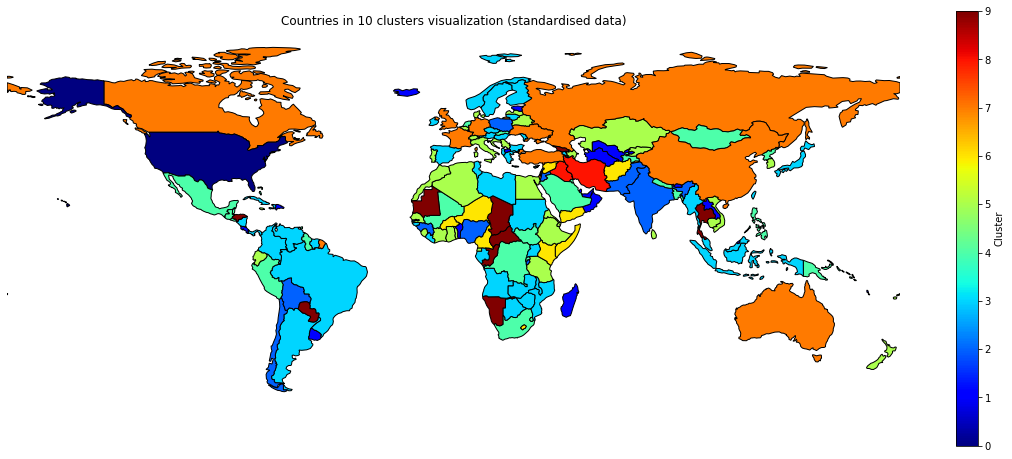
\includegraphics[width=1 \textwidth]{fig/CLUST/10clusterMap_std.png}
        \caption{Mapa z wynikami klasteryzacji. (źródło: opracowanie własne)}
        \label{fig:clust10std}
    \end{figure}

    Aby ułatwić interpretację wyników klasteryzacji poniżej dołączona została mapa~\ref{fig:clustPop} z naniesioną populacją oraz mapa~\ref{fig:clustGDP} z naniesionym PKB na osobę poszczególnych krajów.

    \begin{figure}[ht!]
        \centering
        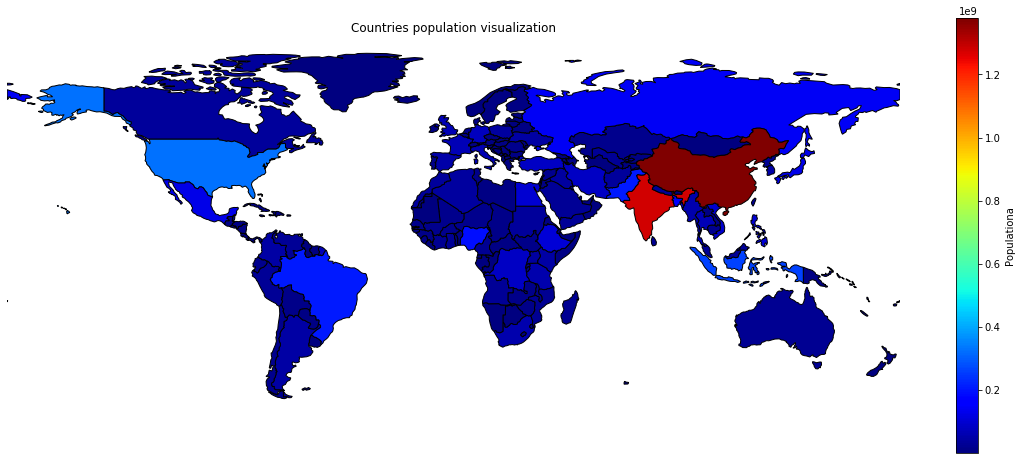
\includegraphics[width=1 \textwidth]{fig/CLUST/population.png}
        \caption{Mapa z populacją krajów. (źródło: opracowanie własne)}
        \label{fig:clustPop}
    \end{figure}

    \begin{figure}[ht!]
        \centering
        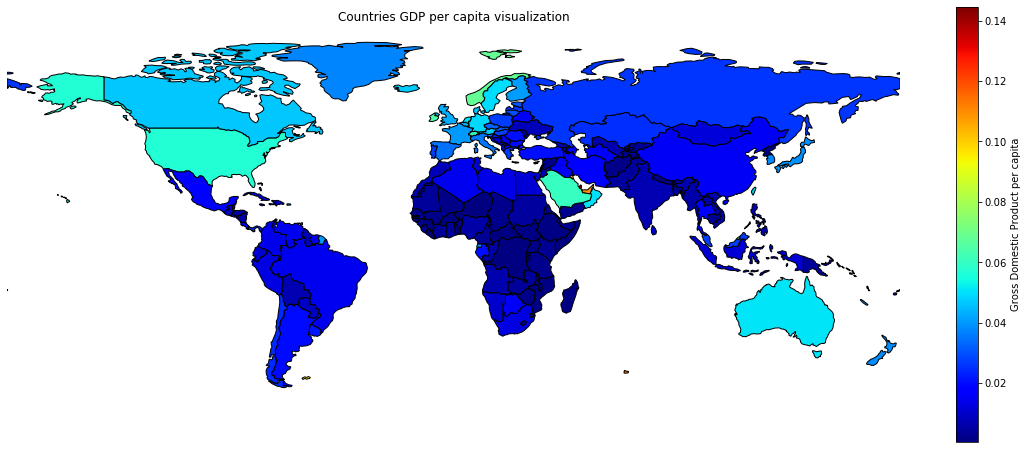
\includegraphics[width=1 \textwidth]{fig/CLUST/gdp.png}
        \caption{Mapa z PKP na osobę. (źródło: opracowanie własne)}
        \label{fig:clustGDP}
    \end{figure}

    \paragraph{Wyniki klasteryzacji w postacji tabelarycznej}
    W tabelach od~\ref{tab:cl0std} do~\ref{tab:cl9std} przedstawione zostały wyniki grupowania ustandaryzowanych próbek.
    Dodatkowo, jak przy danych niestandaryzowanych, zawarto informacje o ilości ludności i PKB na osobę pochodzące z biblioteki GeoPandas~\cite{geopandas}.

    \begin{table}[h!]
        \caption {Klaster 0 - dane standaryzowane} \label{tab:cl0std}
        \begin{tabular}{lllll}
            \hline
            \multicolumn{1}{|l|}{iso\_a3} & \multicolumn{1}{l|}{name} & \multicolumn{1}{l|}{continent} & \multicolumn{1}{l|}{pop\_est} & \multicolumn{1}{l|}{gdp\_per\_cap} \\ \hline
            USA                           & United States of America  & North America                  & 326625791                     & 0.056823
        \end{tabular}
    \end{table}

    \begin{table}[h!]
        \caption {Klaster 1 - dane standaryzowane} \label{tab:cl1std}
        \begin{tabular}{lllll}
            \hline
            \multicolumn{1}{|l|}{iso\_a3} & \multicolumn{1}{l|}{name} & \multicolumn{1}{l|}{continent} & \multicolumn{1}{l|}{pop\_est} & \multicolumn{1}{l|}{gdp\_per\_cap} \\ \hline
            BEN                           & Benin                     & Africa                         & 11038805                      & 0.002202                           \\
            BTN                           & Bhutan                    & Asia                           & 758288                        & 0.008482                           \\
            BRN                           & Brunei                    & Asia                           & 443593                        & 0.076038                           \\
            CRI                           & Costa Rica                & North America                  & 4930258                       & 0.016076                           \\
            DOM                           & Dominican Rep.            & North America                  & 10734247                      & 0.015083                           \\
            EST                           & Estonia                   & Europe                         & 1251581                       & 0.030921                           \\
            ISL                           & Iceland                   & Europe                         & 339747                        & 0.047535                           \\
            LAO                           & Laos                      & Asia                           & 7126706                       & 0.005747                           \\
            LUX                           & Luxembourg                & Europe                         & 594130                        & 0.098867                           \\
            MKD                           & Macedonia                 & Europe                         & 2103721                       & 0.014032                           \\
            MDG                           & Madagascar                & Africa                         & 25054161                      & 0.001471                           \\
            OMN                           & Oman                      & Asia                           & 3424386                       & 0.050549                           \\
            QAT                           & Qatar                     & Asia                           & 2314307                       & 0.144536                           \\
            TKM                           & Turkmenistan              & Asia                           & 5351277                       & 0.017700                           \\
            ARE                           & United Arab Emirates      & Asia                           & 6072475                       & 0.109873                           \\
            URY                           & Uruguay                   & South America                  & 3360148                       & 0.021800                           \\
            UZB                           & Uzbekistan                & Asia                           & 29748859                      & 0.006800                           \\
            VUT                           & Vanuatu                   & Oceania                        & 282814                        & 0.002556
        \end{tabular}
    \end{table}

    \begin{table}[h!]
        \caption {Klaster 2 - dane standaryzowane} \label{tab:cl2std}
        \begin{tabular}{lllll}
            \hline
            \multicolumn{1}{|l|}{iso\_a3} & \multicolumn{1}{l|}{name} & \multicolumn{1}{l|}{continent} & \multicolumn{1}{l|}{pop\_est} & \multicolumn{1}{l|}{gdp\_per\_cap} \\ \hline
            BOL                           & Bolivia                   & South America                  & 11138234                      & 0.007034                           \\
            BDI                           & Burundi                   & Africa                         & 11466756                      & 0.000688                           \\
            CHL                           & Chile                     & South America                  & 17789267                      & 0.024515                           \\
            GMB                           & Gambia                    & Africa                         & 2051363                       & 0.001651                           \\
            GIN                           & Guinea                    & Africa                         & 12413867                      & 0.001295                           \\
            IND                           & India                     & Asia                           & 1281935911                    & 0.006803                           \\
            JOR                           & Jordan                    & Asia                           & 10248069                      & 0.008410                           \\
            LBN                           & Lebanon                   & Asia                           & 6229794                       & 0.013670                           \\
            NGA                           & Nigeria                   & Africa                         & 190632261                     & 0.005713                           \\
            PAK                           & Pakistan                  & Asia                           & 204924861                     & 0.004822                           \\
            PSE                           & Palestine                 & Asia                           & 4543126                       & 0.004671                           \\
            POL                           & Poland                    & Europe                         & 38476269                      & 0.027342
        \end{tabular}
    \end{table}

    \begin{table}[h!]
        \caption {Klaster 3 - dane standaryzowane} \label{tab:cl3std}
        \begin{tabular}{lllll}
            \hline
            \multicolumn{1}{|l|}{iso\_a3} & \multicolumn{1}{l|}{name} & \multicolumn{1}{l|}{continent} & \multicolumn{1}{l|}{pop\_est} & \multicolumn{1}{l|}{gdp\_per\_cap} \\ \hline
            ALB                           & Albania                   & Europe                         & 3047987                       & 0.011122                           \\
            AGO                           & Angola                    & Africa                         & 29310273                      & 0.006448                           \\
            ARG                           & Argentina                 & South America                  & 44293293                      & 0.019854                           \\
            ARM                           & Armenia                   & Asia                           & 3045191                       & 0.008637                           \\
            AUT                           & Austria                   & Europe                         & 8754413                       & 0.047587                           \\
            BWA                           & Botswana                  & Africa                         & 2214858                       & 0.016209                           \\
            BRA                           & Brazil                    & South America                  & 207353391                     & 0.014859                           \\
            BGR                           & Bulgaria                  & Europe                         & 7101510                       & 0.020151                           \\
            COL                           & Colombia                  & South America                  & 47698524                      & 0.014424                           \\
            CUB                           & Cuba                      & North America                  & 11147407                      & 0.011922                           \\
            CYP                           & Cyprus                    & Asia                           & 1221549                       & 0.023953                           \\
            CYP                           & Cyprus                    & Asia                           & 1221549                       & 0.023953                           \\
            CZE                           & Czechia                   & Europe                         & 10674723                      & 0.032872                           \\
            FIN                           & Finland                   & Europe                         & 5491218                       & 0.040817                           \\
            GAB                           & Gabon                     & Africa                         & 1772255                       & 0.020302                           \\
            GRC                           & Greece                    & Europe                         & 10768477                      & 0.026977                           \\
            GNB                           & Guinea-Bissau             & Africa                         & 1792338                       & 0.001591                           \\
            HTI                           & Haiti                     & North America                  & 10646714                      & 0.001817                           \\
            HUN                           & Hungary                   & Europe                         & 9850845                       & 0.027165                           \\
            IDN                           & Indonesia                 & Asia                           & 260580739                     & 0.011620                           \\
            IRL                           & Ireland                   & Europe                         & 5011102                       & 0.064257                           \\
            JPN                           & Japan                     & Asia                           & 126451398                     & 0.039003                           \\
            LBR                           & Liberia                   & Africa                         & 4689021                       & 0.000828                           \\
            LBY                           & Libya                     & Africa                         & 6653210                       & 0.013661                           \\
            LTU                           & Lithuania                 & Europe                         & 2823859                       & 0.030320                           \\
            MWI                           & Malawi                    & Africa                         & 19196246                      & 0.001104                           \\
            MYS                           & Malaysia                  & Asia                           & 31381992                      & 0.027500                           \\
            MDA                           & Moldova                   & Europe                         & 3474121                       & 0.005337                           \\
            MOZ                           & Mozambique                & Africa                         & 26573706                      & 0.001317                           \\
            MMR                           & Myanmar                   & Asia                           & 55123814                      & 0.005644                           \\
            CYP                           & N. Cyprus                 & Asia                           & 265100                        & 0.013580                           \\
            CYP                           & N. Cyprus                 & Asia                           & 265100                        & 0.013580                           \\
            NIC                           & Nicaragua                 & North America                  & 6025951                       & 0.005568                           \\
            NOR                           & Norway                    & Europe                         & 5320045                       & 0.068552                           \\
            PAN                           & Panama                    & North America                  & 3753142                       & 0.024811                           \\
            ESP                           & Spain                     & Europe                         & 48958159                      & 0.034519                           \\
            SDN                           & Sudan                     & Africa                         & 37345935                      & 0.004721                           \\
            SUR                           & Suriname                  & South America                  & 591919                        & 0.014439                           \\
            SWE                           & Sweden                    & Europe                         & 9960487                       & 0.050008                           \\
            TWN                           & Taiwan                    & Asia                           & 23508428                      & 0.047940                           \\
            TUN                           & Tunisia                   & Africa                         & 11403800                      & 0.011470                           \\
            UGA                           & Uganda                    & Africa                         & 39570125                      & 0.002146                           \\
            VEN                           & Venezuela                 & South America                  & 31304016                      & 0.014969                           \\
            ZMB                           & Zambia                    & Africa                         & 15972000                      & 0.004080                           \\
            ZWE                           & Zimbabwe                  & Africa                         & 13805084                      & 0.002052
        \end{tabular}
    \end{table}

    \begin{table}[h!]
        \caption {Klaster 4 - dane standaryzowane} \label{tab:cl4std}
        \begin{tabular}{lllll}
            \hline
            \multicolumn{1}{|l|}{iso\_a3} & \multicolumn{1}{l|}{name} & \multicolumn{1}{l|}{continent} & \multicolumn{1}{l|}{pop\_est} & \multicolumn{1}{l|}{gdp\_per\_cap} \\ \hline
            BHS                           & Bahamas                   & North America                  & 329988                        & 0.027474                           \\
            BGD                           & Bangladesh                & Asia                           & 157826578                     & 0.003982                           \\
            BLZ                           & Belize                    & North America                  & 360346                        & 0.008570                           \\
            COD                           & Dem. Rep. Congo           & Africa                         & 83301151                      & 0.000792                           \\
            SLV                           & El Salvador               & North America                  & 6172011                       & 0.008877                           \\
            GTM                           & Guatemala                 & North America                  & 15460732                      & 0.008525                           \\
            GUY                           & Guyana                    & South America                  & 737718                        & 0.008259                           \\
            KWT                           & Kuwait                    & Asia                           & 2875422                       & 0.104715                           \\
            MLI                           & Mali                      & Africa                         & 17885245                      & 0.002130                           \\
            MEX                           & Mexico                    & North America                  & 124574795                     & 0.018519                           \\
            MNG                           & Mongolia                  & Asia                           & 3068243                       & 0.012059                           \\
            NPL                           & Nepal                     & Asia                           & 29384297                      & 0.002434                           \\
            NLD                           & Netherlands               & Europe                         & 17084719                      & 0.050970                           \\
            PRK                           & North Korea               & Asia                           & 25248140                      & 0.001584                           \\
            PNG                           & Papua New Guinea          & Oceania                        & 6909701                       & 0.004055                           \\
            PER                           & Peru                      & South America                  & 31036656                      & 0.013223                           \\
            PHL                           & Philippines               & Asia                           & 104256076                     & 0.007692                           \\
            RWA                           & Rwanda                    & Africa                         & 11901484                      & 0.001846                           \\
            SSD                           & S. Sudan                  & Africa                         & 13026129                      & 0.001603                           \\
            SAU                           & Saudi Arabia              & Asia                           & 28571770                      & 0.060584                           \\
            SVK                           & Slovakia                  & Europe                         & 5445829                       & 0.030996                           \\
            SLB                           & Solomon Is.               & Oceania                        & 647581                        & 0.001850                           \\
            ZAF                           & South Africa              & Africa                         & 54841552                      & 0.013477                           \\
            TJK                           & Tajikistan                & Asia                           & 8468555                       & 0.003048                           \\
            TTO                           & Trinidad and Tobago       & North America                  & 1218208                       & 0.035766                           \\
            SWZ                           & eSwatini                  & Africa                         & 1467152                       & 0.007538
        \end{tabular}
    \end{table}

    \begin{table}[h!]
        \caption {Klaster 5 - dane standaryzowane} \label{tab:cl5std}
        \begin{tabular}{lllll}
            \hline
            \multicolumn{1}{|l|}{iso\_a3} & \multicolumn{1}{l|}{name} & \multicolumn{1}{l|}{continent} & \multicolumn{1}{l|}{pop\_est} & \multicolumn{1}{l|}{gdp\_per\_cap} \\ \hline
            DZA                           & Algeria                   & Africa                         & 40969443                      & 0.014875                           \\
            AZE                           & Azerbaijan                & Asia                           & 9961396                       & 0.016855                           \\
            BLR                           & Belarus                   & Europe                         & 9549747                       & 0.017320                           \\
            BEL                           & Belgium                   & Europe                         & 11491346                      & 0.044259                           \\
            KHM                           & Cambodia                  & Asia                           & 16204486                      & 0.003637                           \\
            HRV                           & Croatia                   & Europe                         & 4292095                       & 0.021957                           \\
            CIV                           & Côte d'Ivoire             & Africa                         & 24184810                      & 0.003602                           \\
            DNK                           & Denmark                   & Europe                         & 5605948                       & 0.047236                           \\
            DJI                           & Djibouti                  & Africa                         & 865267                        & 0.003866                           \\
            ECU                           & Ecuador                   & South America                  & 16290913                      & 0.011196                           \\
            EGY                           & Egypt                     & Africa                         & 97041072                      & 0.011387                           \\
            GNQ                           & Eq. Guinea                & Africa                         & 778358                        & 0.040817                           \\
            ERI                           & Eritrea                   & Africa                         & 5918919                       & 0.001549                           \\
            ETH                           & Ethiopia                  & Africa                         & 105350020                     & 0.001658                           \\
            FJI                           & Fiji                      & Oceania                        & 920938                        & 0.009093                           \\
            GHA                           & Ghana                     & Africa                         & 27499924                      & 0.004393                           \\
            ITA                           & Italy                     & Europe                         & 62137802                      & 0.035743                           \\
            JAM                           & Jamaica                   & North America                  & 2990561                       & 0.008490                           \\
            KAZ                           & Kazakhstan                & Asia                           & 18556698                      & 0.024827                           \\
            KGZ                           & Kyrgyzstan                & Asia                           & 5789122                       & 0.003629                           \\
            LVA                           & Latvia                    & Europe                         & 1944643                       & 0.026046                           \\
            MAR                           & Morocco                   & Africa                         & 33986655                      & 0.008321                           \\
            NZL                           & New Zealand               & Oceania                        & 4510327                       & 0.038756                           \\
            PRT                           & Portugal                  & Europe                         & 10839514                      & 0.027409                           \\
            SEN                           & Senegal                   & Africa                         & 14668522                      & 0.002708                           \\
            SRB                           & Serbia                    & Europe                         & 7111024                       & 0.014316                           \\
            SLE                           & Sierra Leone              & Africa                         & 6163195                       & 0.001726                           \\
            KOR                           & South Korea               & Asia                           & 51181299                      & 0.037690                           \\
            LKA                           & Sri Lanka                 & Asia                           & 22409381                      & 0.010563                           \\
            CHE                           & Switzerland               & Europe                         & 8236303                       & 0.060258                           \\
            TZA                           & Tanzania                  & Africa                         & 53950935                      & 0.002791                           \\
            TGO                           & Togo                      & Africa                         & 7965055                       & 0.001458                           \\
            VNM                           & Vietnam                   & Asia                           & 96160163                      & 0.006187
        \end{tabular}
    \end{table}

    \begin{table}[h!]
        \caption {Klaster 6 - dane standaryzowane} \label{tab:cl6std}
        \begin{tabular}{lllll}
            \hline
            \multicolumn{1}{|l|}{iso\_a3} & \multicolumn{1}{l|}{name} & \multicolumn{1}{l|}{continent} & \multicolumn{1}{l|}{pop\_est} & \multicolumn{1}{l|}{gdp\_per\_cap} \\ \hline
            AFG                           & Afghanistan               & Asia                           & 34124811                      & 0.001878                           \\
            BFA                           & Burkina Faso              & Africa                         & 20107509                      & 0.001641                           \\
            CMR                           & Cameroon                  & Africa                         & 24994885                      & 0.003090                           \\
            KEN                           & Kenya                     & Africa                         & 47615739                      & 0.003207                           \\
            LSO                           & Lesotho                   & Africa                         & 1958042                       & 0.003074                           \\
            NER                           & Niger                     & Africa                         & 19245344                      & 0.001047                           \\
            SOM                           & Somalia                   & Africa                         & 7531386                       & 0.000627                           \\
            SYR                           & Syria                     & Asia                           & 18028549                      & 0.002789                           \\
            YEM                           & Yemen                     & Asia                           & 28036829                      & 0.002620
        \end{tabular}
    \end{table}

    \begin{table}[h!]
        \caption {Klaster 7 - dane standaryzowane} \label{tab:cl7std}
        \begin{tabular}{lllll}
            \hline
            \multicolumn{1}{|l|}{iso\_a3} & \multicolumn{1}{l|}{name} & \multicolumn{1}{l|}{continent} & \multicolumn{1}{l|}{pop\_est} & \multicolumn{1}{l|}{gdp\_per\_cap} \\ \hline
            AUS                           & Australia                 & Oceania                        & 23232413                      & 0.051178                           \\
            CAN                           & Canada                    & North America                  & 35623680                      & 0.046991                           \\
            CHN                           & China                     & Asia                           & 1379302771                    & 0.015327                           \\
            FRA                           & France                    & Europe                         & 67106161                      & 0.040220                           \\
            DEU                           & Germany                   & Europe                         & 80594017                      & 0.049371                           \\
            ISR                           & Israel                    & Asia                           & 8299706                       & 0.035784                           \\
            RUS                           & Russia                    & Europe                         & 142257519                     & 0.026325                           \\
            TUR                           & Turkey                    & Asia                           & 80845215                      & 0.020657                           \\
            UKR                           & Ukraine                   & Europe                         & 44033874                      & 0.008007                           \\
            GBR                           & United Kingdom            & Europe                         & 64769452                      & 0.043045
        \end{tabular}
    \end{table}

    \begin{table}[h!]
        \caption {Klaster 8 - dane standaryzowane} \label{tab:cl8std}
        \begin{tabular}{lllll}
            \hline
            \multicolumn{1}{|l|}{iso\_a3} & \multicolumn{1}{l|}{name} & \multicolumn{1}{l|}{continent} & \multicolumn{1}{l|}{pop\_est} & \multicolumn{1}{l|}{gdp\_per\_cap} \\ \hline
            IRN                           & Iran                      & Asia                           & 82021564                      & 0.017788                           \\
            IRQ                           & Iraq                      & Asia                           & 39192111                      & 0.015225
        \end{tabular}
    \end{table}

    \begin{table}[h!]
        \caption {Klaster 9 - dane standaryzowane} \label{tab:cl9std}
        \begin{tabular}{lllll}
            \hline
            \multicolumn{1}{|l|}{iso\_a3} & \multicolumn{1}{l|}{name} & \multicolumn{1}{l|}{continent} & \multicolumn{1}{l|}{pop\_est} & \multicolumn{1}{l|}{gdp\_per\_cap} \\ \hline
            CAF                           & Central African Rep.      & Africa                         & 5625118                       & 0.000570                           \\
            TCD                           & Chad                      & Africa                         & 12075985                      & 0.002533                           \\
            COG                           & Congo                     & Africa                         & 4954674                       & 0.006109                           \\
            GEO                           & Georgia                   & Asia                           & 4926330                       & 0.007565                           \\
            HND                           & Honduras                  & North America                  & 9038741                       & 0.004778                           \\
            MRT                           & Mauritania                & Africa                         & 3758571                       & 0.004446                           \\
            NAM                           & Namibia                   & Africa                         & 2484780                       & 0.010460                           \\
            PRY                           & Paraguay                  & South America                  & 6943739                       & 0.009313                           \\
            THA                           & Thailand                  & Asia                           & 68414135                      & 0.016970
        \end{tabular}
    \end{table}

    Zarówno dla danych nie poddanych oraz poddanych standaryzacji Stany Zjednoczono otrzymały własny klaster -~\ref{tab:cl7} oraz ~\ref{tab:cl0std}.
    Jest to spowodowane znaczącą przewagą ilości zdarzeń w porównaniu z innymi krajami.

    Dla danych standaryzowanych Polska jest jedynym krajem europejskim w klastrze~\ref{tab:cl2std}.
    Irak oraz Iran otrzymały własny klaster~\ref{tab:cl8std}.
    Wyróżnia się mniejsza grupa~\ref{tab:cl7std} w której znalazły się między innymi: Chiny, Francja, Niemcy, Rosja, Wielka Brytania.


    \chapter{Podsumowanie}
    W niniejszej części zostaną opisane wnioski z pracy według kolejności wcześniej przedstawionych rozdziałów.


    \section{Dalsze kierunki rozwoju}
    W tej części zostaną opisane możliwe kierunki rozwoju pracy.

    \paragraph{Analiza pod kątem COVID-19}

    \paragraph{Analiza pod kątem grup etnicznych}

    \paragraph{Analiza pod kątem grup religijnych}


    \inputencoding{utf8}

    \newpage
    \addcontentsline{toc}{chapter}{Bibliografia}
    \printbibliography[title={Bibliografia}]

\end{document}
